% =====================================================================
% presentazione.tex
% Presentazione della tesi "Selezione Dinamica della Dimensione del
% Campione in Metodi di Ottimizzazione per il Machine Learning".
%
% Riorganizzata come traccia di esposizione: contesto e stato
% dell'arte (SGD, metodi a varianza ridotta SVRG/SAGA con schemi),
% quindi CCV, algoritmi a campionamento dinamico, teoria,
% esperimenti, riuso del mini-batch, conclusioni.
%
% Compilazione:
%   cd presentazione
%   latexmk -pdf presentazione.tex
% =====================================================================
\documentclass[aspectratio=169,11pt]{beamer}

% ---- pacchetti ----
\usepackage[T1]{fontenc}
\usepackage[utf8]{inputenc}
\usepackage[italian]{babel}
\usepackage{amsmath, amssymb, bm}
\usepackage{graphicx}
\usepackage{booktabs}
\usepackage{colortbl}
% --- Scala log per le tabelle colorate (identica a tesi_finale, Sez. 6) ---
% Ancoraggi robusti agli outlier: min = 1° percentile errori (7.4e-3),
% max = 1.4142 (errore iniziale). I valori sotto il 1° percentile
% (fino a 1.0991e-14, precisione macchina di BB-CCV) si saturano in verde.
\def\minLog{-2.130}
\def\maxLog{0.1505}
\definecolor{lowcolor}{RGB}{190,255,190}
\definecolor{highcolor}{RGB}{140,0,0}
% \colorcell{mantissa}{esponente}: sfondo cella = errore m*10^e, scala log globale
\newcommand{\colorcell}[2]{%
  \pgfmathparse{log10(#1)+(#2)}%
  \let\colcellLog\pgfmathresult%
  \pgfmathparse{(\colcellLog-\minLog)/(\maxLog-\minLog)}%
  \let\colcellT\pgfmathresult%
  \pgfmathparse{max(0,min(1,\colcellT))}%
  \let\colcellT\pgfmathresult%
  \pgfmathsetmacro{\colcellR}{round(190+(140-190)*\colcellT)}%
  \pgfmathsetmacro{\colcellG}{round(255+(0-255)*\colcellT)}%
  \pgfmathsetmacro{\colcellB}{round(190+(0-190)*\colcellT)}%
  \edef\colcellCC{\noexpand\cellcolor[RGB]{\colcellR,\colcellG,\colcellB}}%
  \colcellCC{\color{black}$#1\times10^{#2}$}%
}

% ---- font professionali (Times, stile tesi) ----
\usepackage{newtxtext}
\usepackage{newtxmath}
\renewcommand{\familydefault}{\rmdefault}
\graphicspath{{immagini/}}

% ---- colori (tema scuro, sfondo nero) ----
\definecolor{sfondo}{RGB}{0,0,0}          % sfondo nero
\definecolor{testo}{RGB}{255,255,255}     % testo bianco
\definecolor{acc}{RGB}{245,185,66}        % accento ambra (titoli)
\definecolor{acc2}{RGB}{138,180,248}      % accento azzurro (secondario)
\definecolor{grigio}{RGB}{176,176,176}    % sottotitoli / note

\setbeamercolor{background canvas}{bg=sfondo}
\setbeamercolor{normal text}{fg=testo}
\setbeamercolor{frametitle}{fg=acc}
\setbeamercolor{title}{fg=acc}
\setbeamercolor{subtitle}{fg=grigio}
\setbeamercolor{itemize item}{fg=acc}
\setbeamercolor{itemize subitem}{fg=acc2}
\setbeamercolor{enumerate item}{fg=acc}
\setbeamercolor{footline}{fg=testo}

% ogni formula (inline e display) in bianco
\AtBeginDocument{\everymath{\color{testo}}}

% struttura e titoli in serif (Times)
\usefonttheme{professionalfonts}
\setbeamerfont{title}{family=\rmfamily,series=\bfseries}
\setbeamerfont{frametitle}{family=\rmfamily,series=\bfseries}
\setbeamerfont{subtitle}{family=\rmfamily}

% marcatori di lista
\setbeamertemplate{itemize item}{\textbullet}
\setbeamertemplate{itemize subitem}{\textendash}

% niente simboli di navigazione
\setbeamertemplate{navigation symbols}{}

% piè di pagina: solo numero di pagina a destra
\setbeamertemplate{footline}{%
  \leavevmode\hbox{%
    \begin{beamercolorbox}[wd=\paperwidth,ht=2.6ex,dp=1.2ex,right]{footline}%
      \small\insertframenumber/\inserttotalframenumber\hspace*{1.6ex}%
    \end{beamercolorbox}}%
  \vskip0pt}

% comodità per il sottotitolo "Dalla tesi ..."
\newcommand{\fonte}[1]{\par\vspace{-0.15cm}{\small\color{grigio}#1}\par}

% ---- migliorie grafiche ----
% parola chiave in ambra (grassetto colorato)
\newcommand{\kw}[1]{\textcolor{acc}{\textbf{#1}}}

% titolo con riga colorata sotto
\setbeamertemplate{frametitle}{%
  \noindent\usebeamerfont{frametitle}\color{acc}\insertframetitle\par
  \vskip-0.30ex
  {\color{acc}\hrule height 0.6pt}\vskip0.25ex}

% piè di pagina: barra di avanzamento + numero pagina
\setbeamertemplate{footline}{%
  \leavevmode\hbox{%
    \begin{beamercolorbox}[wd=\paperwidth,ht=3.0ex,dp=1.1ex]{footline}%
      \hspace*{1.2ex}%
      {\color{acc}\rule{\dimexpr(\paperwidth-3ex)*\insertframenumber/\inserttotalframenumber}{1.4pt}}%
      \hfill{\small\insertframenumber/\inserttotalframenumber\hspace*{1.6ex}}%
    \end{beamercolorbox}}%
  \vskip0pt}

% riquadro "take-away" / risultato chiave
\newcommand{\takeaway}[1]{%
  \begin{center}
    \fcolorbox{acc}{sfondo}{\parbox{0.9\textwidth}{\centering\small\kw{#1}}}
  \end{center}}

\title{Selezione Dinamica della Dimensione del Campione}
\subtitle{in Metodi di Ottimizzazione per il Machine Learning}
\author{Alessandro Lo Curcio}

\begin{document}

% =====================================================================
% SLIDE 1 — Titolo + abstract
% =====================================================================
\begin{frame}
  \begin{center}
    {\LARGE\bfseries\color{acc} Selezione Dinamica della Dimensione del Campione}\\[0.3cm]
    {\large in Metodi di Ottimizzazione per il Machine Learning}\\[0.6cm]
    \textcolor{acc2}{\rule{0.7\textwidth}{0.8pt}}\\[0.5cm]
  \end{center}
  \small
  La tesi presenta la selezione dinamica della dimensione del campione
  negli algoritmi di ottimizzazione per il machine learning su larga scala,
  fondandosi sul lavoro di Byrd, Chin, Nocedal e Wu (2012). L'idea centrale:
  invece di fissare a priori la dimensione del batch, si decide durante
  l'algoritmo se e quando aumentarla, guidandosi da stime statistiche della
  varianza del gradiente stocastico. Il lavoro offre un'analisi teorica
  completa della convergenza, il miglioramento di alcuni risultati mediante
  disuguaglianze più strette e un'implementazione Python dei quattro algoritmi
  principali: Dynamic GD, Newton-CG, estensione $L_1$ e BB-CCV, con
  un'applicazione web interattiva per la sperimentazione.
\end{frame}

% =====================================================================
% SLIDE 2 — Contesto: ottimizzazione su larga scala
% =====================================================================
\begin{frame}{Contesto: ottimizzazione su larga scala}
  \begin{itemize}
    \item Obiettivo: minimizzare la perdita empirica
      \[
        J(w) = \frac{1}{N}\sum_{i=1}^{N}\ell(w;i),
        \qquad w\in\mathbb{R}^m
      \]
      con $N \approx 10^6$--$10^9$ esempi e $m$ grande: il gradiente completo
      $\nabla J(w)$ costa $O(Nm)$ per iterazione, proibitivo.
    \item Mini-batch $\mathcal{S}_k$ di dimensione $n_k$: stima
      $g_k=\nabla J_{\mathcal{S}_k}(w_k)$, costo $O(n_k m)$.
      Se $n_k\ll N$ le iterazioni sono economiche.
    \item Compromesso classico (Bottou--Bousquet, 2008):
      batch piccolo = stima rumorosa; batch grande = stima accurata ma costo
      proporzionale alla dimensione.
    \item Nei metodi classici $n_k$ è \textbf{fissata a priori}; questa tesi
      analizza la proposta di renderla \textbf{dinamica} durante le
      iterazioni (Byrd, Chin, Nocedal e Wu, 2012).
  \end{itemize}
\end{frame}

% =====================================================================
% SLIDE 3 — Stato dell'arte: SGD e il problema della varianza
% =====================================================================
\begin{frame}{Stato dell'arte: SGD e il problema della varianza}
  \begin{itemize}
    \item SGD (Robbins--Monro, 1951): aggiornamento su un singolo esempio
      (o un piccolo batch),
      $w_{k+1}=w_k-\alpha_k\nabla\ell(w_k;i_k)$, con
      $\mathbb{E}[\nabla\ell(w_k;i)]=\nabla J(w_k)$: stimatore
      \emph{non distorto}, costo per iterazione indipendente da $N$.
    \item Ma la varianza $\mathrm{Var}[\nabla\ell(w;i)]$ \textbf{non} tende a
      zero vicino all'ottimo: quando $\nabla J(w)\to 0$ il rumore domina e
      limita la precisione raggiungibile.
    \item Conseguenze pratiche: a passo fisso si resta in un intorno
      dell'ottimo (precisione limitata); a passo $\alpha_k\to 0$ la
      convergenza rallenta.
    \item Su larga scala conta il \textbf{costo totale} (costo per iterazione
      $\times$ numero di iterazioni), non solo il numero di iterazioni.
    \item Due strade per uscirne: aumentare il campione (costo) oppure
      ridurre la varianza con stimatori migliori.
  \end{itemize}
\end{frame}

% =====================================================================
% SLIDE 4 — Metodi a varianza ridotta: l'idea comune
% =====================================================================
\begin{frame}{Metodi a varianza ridotta: l'idea comune}
  \begin{itemize}
    \item SVRG (\emph{Stochastic Variance Reduced Gradient};
      Johnson--Zhang, 2013) e SAGA (metodo di riduzione della varianza di
      Defazio--Bach--Lacoste-Julien, 2014):
      SGD + \emph{correzione} costruita su quantità globali.
    \item Forma generale dello stimatore corretto:
      \[
        g_k = \nabla\ell(w_k;i_k) - c_k + \mathbb{E}[c_k],
      \]
      che resta non distorto: $\mathbb{E}[g_k]=\nabla J(w_k)$.
    \item Se la correzione $c_k$ è correlata al rumore del gradiente
      stocastico, la varianza di $g_k$ si riduce (idealmente tende a zero
      vicino all'ottimo): \emph{variance reduction}.
    \item Differenza chiave tra i due metodi:
      \begin{itemize}
        \item \textbf{SVRG}: ricalcola periodicamente un gradiente esatto su
          un punto di ancoraggio;
        \item \textbf{SAGA}: mantiene una tavola dei gradienti per-esempio,
          aggiornata a ogni iterazione.
      \end{itemize}
  \end{itemize}
  \fonte{Dalla tesi --- Sez.~4.1 (Lavori Correlati) e Appendice~D (Schemi
    dei metodi a varianza ridotta)}
\end{frame}

% =====================================================================
% SLIDE 5 — Schema SVRG e perché ricampionare ogni m iterazioni
% =====================================================================
\begin{frame}{SVRG: l'ancora e il ricampionamento ogni $t$ iterazioni}
  \small
  \begin{columns}[T]
    \begin{column}{0.56\textwidth}
      \begin{itemize}
        \item Punto di ancoraggio $\bar w$ con gradiente esatto
          $\nabla J(\bar w)$, ricalcolato ogni $t$ iterazioni.
        \item Stimatore non distorto:
          \[
            g_k=\nabla\ell(w_k;i_k)-\nabla\ell(\bar w;i_k)+\nabla J(\bar w)
          \]
        \item \textbf{Idea}: finché $w_k\approx\bar w$, per la regolarità dei
          gradienti $\nabla\ell(w_k;i_k)\approx\nabla\ell(\bar w;i_k)$: i due
          termini stocastici si elidono e resta $g_k\approx\nabla J(\bar w)$:
          poca varianza.
        \item Quando $w_k$ si allontana da $\bar w$ la correzione
          ``invecchia'': il rumore non è più eliso e la varianza ricresce
          $\to$ si aggiorna l'ancora e si ricampiona l'intero dataset.
      \end{itemize}
      \fonte{Dalla tesi --- Appendice~D, Schema SVRG}
    \end{column}
    \begin{column}{0.44\textwidth}
      \begin{center}
        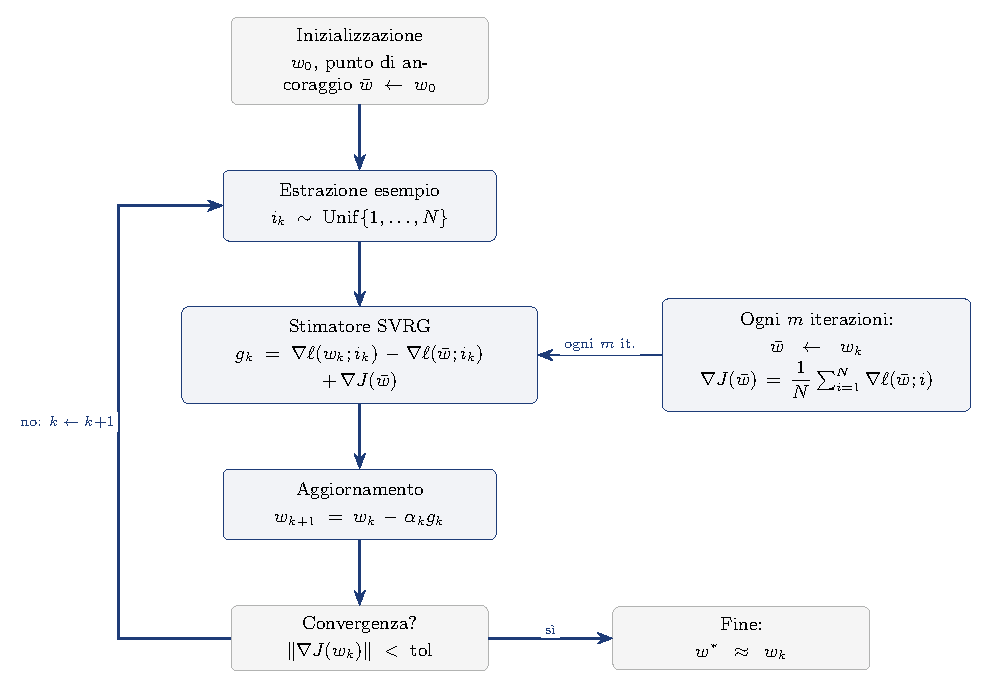
\includegraphics[width=\textwidth,height=0.62\paperheight,keepaspectratio]{schema_svrg.pdf}
      \end{center}
    \end{column}
  \end{columns}
\end{frame}

% =====================================================================
% SLIDE 6 — Schema SAGA
% =====================================================================
\begin{frame}{SAGA: la tavola dei gradienti, nessun ricalcolo globale}
  \begin{columns}[T]
    \begin{column}{0.56\textwidth}
      \begin{itemize}
        \item Tavola $g^{(i)}$: l'ultimo gradiente calcolato per ogni esempio
          $i$; media $\bar g=\frac{1}{N}\sum_i g^{(i)}$ (solo memoria
          $O(Nm)$, nessuna passata completa periodica).
        \item Stimatore:
          \[
            g_k=\nabla\ell(w_k;i_k)-g^{(i_k)}+\bar g
          \]
        \item A ogni iterazione si aggiorna \emph{solo} la voce estratta:
          $g^{(i_k)}\leftarrow\nabla\ell(w_k;i_k)$ e $\bar g$ di
          conseguenza.
        \item Stesso schema di riduzione della varianza di SVRG, ma la
          correzione è sempre ``fresca'' per l'esempio appena campionato.
      \end{itemize}
      \fonte{Dalla tesi --- Appendice~D, Schema SAGA (fig.~saga)}
    \end{column}
    \begin{column}{0.44\textwidth}
      \begin{center}
        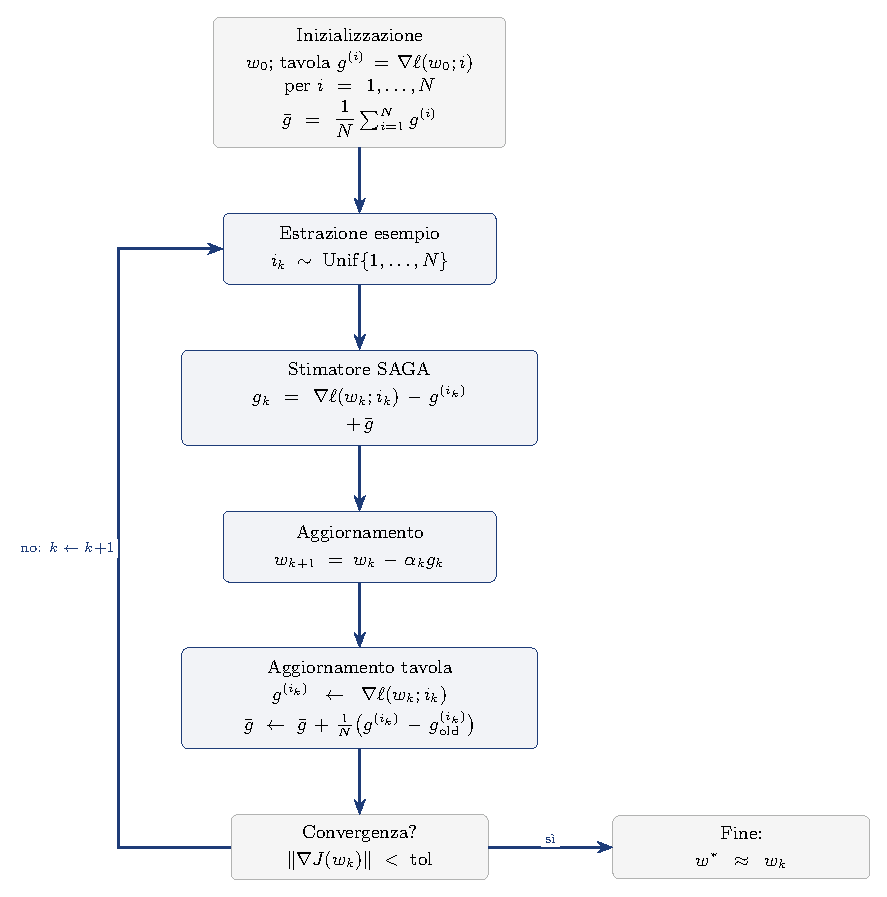
\includegraphics[width=\textwidth,height=0.62\paperheight,keepaspectratio]{schema_saga.pdf}
      \end{center}
    \end{column}
  \end{columns}
\end{frame}

% =====================================================================
% SLIDE 7 — Limiti di SVRG/SAGA e conseguenze per la tesi
% =====================================================================
\begin{frame}{Limiti di SVRG/SAGA e conseguenze per la tesi}
  \begin{itemize}
    \item \textbf{SVRG}: memoria extra minima (solo l'ancora e il suo
      gradiente, $O(m)$); ma ogni $t$ iterazioni va ricalcolato il
      gradiente esatto $\nabla J(\bar w)$ con una passata completa sul
      dataset: costo \emph{temporale} $O(Nm)$ per passata, che per $N$
      molto grande può dominare il costo complessivo.
    \item \textbf{SAGA}: nessuna passata completa periodica, ma
      \emph{memoria} $O(Nm)$ per la tavola dei gradienti (un gradiente
      per ogni esempio): improponibile quando $N\cdot m$ è molto grande.
    \item In entrambi la dimensione del campione è \textbf{fissata a
      priori} (un esempio per iterazione): non è mai adattata
      alle necessità di accuratezza del momento.
    \item Le garanzie di convergenza lineare valgono sotto convessità forte.
    \item \textbf{Conclusione}: rendere \emph{dinamica} la dimensione del
      campione, aumentandola (e ricampionando) quando la stima corrente non
      è abbastanza accurata: è l'approccio di Byrd, Chin, Nocedal e Wu
      (2012), al centro della tesi.
  \end{itemize}
\end{frame}

% =====================================================================
% SLIDE 8 — Varianza del gradiente stimato: definizioni
% =====================================================================
\begin{frame}{La varianza del gradiente stimato: definizioni}
  \small
  \setlength{\abovedisplayskip}{2pt}
  \setlength{\belowdisplayskip}{2pt}
  \setlength{\abovedisplayshortskip}{2pt}
  \setlength{\belowdisplayshortskip}{2pt}
  \begin{itemize}\setlength{\itemsep}{2pt}
    \item Il gradiente sul batch è la \emph{media} dei gradienti per-esempio,
      $g_k=\nabla J_{\mathcal{S}_k}(w_k)
      =\frac{1}{n_k}\sum_{i\in\mathcal{S}_k}\nabla\ell(w_k;i)$, con
      $\mathbb{E}[g_k]=\nabla J(w_k)$ (stimatore non distorto). L'errore
      $e_k=g_k-\nabla J(w_k)$ non è calcolabile; si controlla la \emph{varianza
      dello stimatore}: $\mathbb{E}[\|e_k\|_2^2]=\|\mathrm{Var}(g_k)\|_1$
      (somma delle varianze, componente per componente).
    \item Definizioni: $\mathcal{V}$ è la \emph{varianza della popolazione}
      del gradiente della loss (non calcolabile: servirebbe $\nabla J(w_k)$);
      $\widehat{\mathcal{V}}$ (``v-hat'') è la sua stima \emph{campionaria}
      sul batch corrente, centrata sulla media campionaria $g_k$:
      \[
        \mathcal{V}:=\frac{1}{N}\sum_{i=1}^{N}\bigl(\nabla\ell(w_k;i)-\nabla
        J(w_k)\bigr)^2,\qquad
        \widehat{\mathcal{V}}:=\frac{1}{n_k-1}\sum_{i\in\mathcal{S}_k}
        \bigl(\nabla\ell(w_k;i)-g_k\bigr)^2 ,
      \]
      quadrati e divisioni sempre componente per componente ($\in\mathbb{R}^m$).
  \end{itemize}
  \fonte{Dalla tesi --- Sez.~5.1}
\end{frame}

% =====================================================================
% SLIDE 9 — Varianza dello stimatore: decomposizione
% =====================================================================
\begin{frame}{Varianza dello stimatore: decomposizione}
  \small
  \setlength{\abovedisplayskip}{2pt}
  \setlength{\belowdisplayskip}{2pt}
  \setlength{\abovedisplayshortskip}{2pt}
  \setlength{\belowdisplayshortskip}{2pt}
  \begin{itemize}\setlength{\itemsep}{2pt}
    \item $\widehat{\mathcal{V}}$ (denominatore $n_k-1$) è non distorta,
      $\mathbb{E}[\widehat{\mathcal{V}}]=\mathcal{V}$: stima la
      \emph{dispersione dei singoli gradienti} del batch. Ma $g_k$ è la loro
      \emph{media}; la varianza della media si ricava da quella dei singoli
      con la \emph{decomposizione} (con reinserimento, indipendenza):
      \[
        \mathrm{Var}(g_k)
        =\mathrm{Var}\!\Bigl(\frac{1}{n_k}\sum_{i\in\mathcal{S}_k}
        \nabla\ell(w_k;i)\Bigr)
        =\frac{1}{n_k^2}\sum_{i\in\mathcal{S}_k}\mathrm{Var}\bigl(\nabla
        \ell(w_k;i)\bigr)
        =\frac{\mathcal{V}}{n_k}.
      \]
    \item Senza reinserimento (i batch reali) si aggiunge il \emph{fattore di
      correzione per popolazione finita}:
      \[
        \mathrm{Var}(g_k)=\frac{\mathcal{V}}{n_k}\cdot\frac{N-n_k}{N-1}.
      \]
      La sua dimostrazione è in Appendice (tesi). Per $N\gg n_k$ (condizione
      tipica nel machine learning) il fattore è $\approx1$, quindi vale la
      forma pratica $\mathrm{Var}(g_k)\approx\mathcal{V}/n_k$.
  \end{itemize}
  \fonte{Dalla tesi --- Sez.~5.1; dimostrazione del fattore di correzione per popolazione finita in Appendice}
\end{frame}

% =====================================================================
% SLIDE 10 — Campionamento dinamico e CCV
% =====================================================================
\begin{frame}{Campionamento dinamico: la Condizione di Controllo della Varianza}
  \begin{itemize}
    \item Si parte da un batch piccolo: iterazioni economiche; il batch
      cresce solo quando la stima del gradiente non è abbastanza accurata.
    \item Criterio (CCV): la varianza stimata dello stimatore del gradiente
      deve essere piccola rispetto alla norma del gradiente stimato:
      \[
        \frac{\|\widehat{\mathcal{V}}\|_1}{n_k}
        \;\le\; \theta^2\,\|g_k\|_2^2,
        \qquad \theta\in(0,1)
      \]
    \item Se la CCV è violata si ricampiona con un batch più grande:
      \[
        n_k^{\mathrm{new}}
        \;=\; \left\lceil
        \frac{\|\widehat{\mathcal{V}}\|_1}{\theta^2\,\|g_k\|_2^2}
        \right\rceil
      \]
    \item Profilo a ``scalini''; $\theta$ piccolo $\to$ si aumenta presto
      (batch accurati), $\theta$ grande $\to$ batch piccolo più a lungo.
    \item Nessuna stima di $\kappa$ né regola geometrica a priori: la
      crescita è guidata dai dati.
  \end{itemize}
  \fonte{Dalla tesi --- Sez.~5.1 (Byrd, Chin, Nocedal e Wu, 2012)}
\end{frame}

% =====================================================================
% SLIDE 11 — Direzione di discesa: livello puntuale e garanzia in media
% =====================================================================
\begin{frame}{Direzione di discesa: livello puntuale e garanzia in media}
  \small
  \begin{itemize}\setlength{\itemsep}{3pt}
    \item \textbf{Livello puntuale (deterministico).} Se per il batch corrente vale la condizione di accuratezza
      $\|e_k\|_2\le\theta\|g_k\|_2$ ($e_k=g_k-\nabla J(w_k)$), allora $-g_k$ \`e di discesa per $J$: per
      Cauchy--Schwarz,
      \[
        \nabla J(w_k)^\top g_k
        =\|g_k\|_2^2-e_k^\top g_k
        \;\ge\; \|g_k\|_2^2-\|e_k\|_2\|g_k\|_2
        \;\ge\; (1-\theta)\|g_k\|_2^2 > 0 .
      \]
      \`E una condizione \emph{sufficiente e puntuale}: ipotesi dell'analisi deterministica, non una conseguenza
      della CCV.
    \item \textbf{Livello CCV (in aspettativa).} La CCV controlla la \emph{varianza} dello stimatore
      ($\|\widehat{\mathcal{V}}\|_1/n_k\le\theta^2\|g_k\|_2^2$), non l'errore del singolo mini-batch: non garantisce
      la discesa a ogni iterazione.
    \item \textbf{Garanzia in media.} $g_k$ \`e non distorto, $\mathbb{E}[g_k]=\nabla J(w_k)$, quindi
      \[
        \mathbb{E}\bigl[\nabla J(w_k)^\top g_k\bigr]
        =\nabla J(w_k)^\top\mathbb{E}[g_k]
        =\|\nabla J(w_k)\|_2^2 > 0,
      \]
      e la CCV tiene sotto controllo le fluttuazioni (base dell'analisi di convergenza in media).
  \end{itemize}
  \fonte{Dalla tesi --- Sez.~5.1: condizione puntuale (deterministica), CCV (in aspettativa) e garanzia in media}
\end{frame}

% =====================================================================
% SLIDE 12 — I quattro algoritmi
% =====================================================================
\begin{frame}{I quattro algoritmi a campionamento dinamico}
  \begin{itemize}
    \item \textbf{Dynamic GD}: gradiente su campione dinamico con CCV e line
      search di Wolfe (base del metodo).
    \item \textbf{Newton-CG}: Hessiana sottocampionata
      ($|\mathcal{H}|=R\,|\mathcal{S}|$) e criterio di arresto adattivo del
      CG interno, basato sulla varianza dei prodotti Hessiana-vettore: niente
      iterazioni interne sprecate quando l'Hessiana è limitata dal
      sottocampionamento.
    \item \textbf{Newton-CG $L_1$}: gradiente generalizzato, identificazione
      dell'active set e line search proiettata (soluzioni sparse).
    \item \textbf{BB-CCV}: passo di Barzilai--Borwein con campionamento
      dinamico (line search di Armijo).
    \item Tutti implementati in Python (Appendice~B) e nell'app web
      interattiva; per ognuno, lo schema seguente mostra il flusso con la
      CCV come decisione centrale.
  \end{itemize}
\end{frame}

% =====================================================================
% SLIDE 13 — Condizioni di Wolfe (con $h=\alpha d$)
% =====================================================================
\begin{frame}{Condizioni di Wolfe (con $h=\alpha d$)}
  \footnotesize
  \setlength{\abovedisplayskip}{1pt}
  \setlength{\belowdisplayskip}{1pt}
  \setlength{\abovedisplayshortskip}{1pt}
  \setlength{\belowdisplayshortskip}{1pt}
  \begin{itemize}\setlength{\itemsep}{1pt}
    \item $h=\alpha d$ è lo spostamento lungo una direzione di discesa:
      $\nabla f(x)^Th<0$, quindi nelle formule i due membri sono negativi.
    \item \textbf{Armijo} (prima condizione di Wolfe): la caduta deve essere
      ``sufficiente'',
      \[
        \boxed{\,f(x+h)-f(x)\le c_1\,\nabla f(x)^Th\,},\qquad 0<c_1<1.
      \]
      Moltiplicando per $-1$: la \emph{caduta effettiva} deve essere almeno
      la frazione $c_1$ della caduta lineare prevista dal gradiente.
      Impedisce passi troppo corti o scarsi.
    \item \textbf{Curvatura di Wolfe}: la pendenza finale non deve essere
      troppo ripida,
      \[
        \boxed{\,\nabla f(x+h)^Th\ge c_2\,\nabla f(x)^Th\,},\qquad c_1<c_2<1.
      \]
      Moltiplicando per $-1$: la \emph{pendenza residua} (in valore assoluto)
      deve essere al più la frazione $c_2$ di quella iniziale. Se è ancora
      molto negativa, $f$ continua a scendere: si può allungare il passo.
      Impedisce di fermarsi troppo presto.
  \end{itemize}
  \vspace{0.03cm}
  \begin{center}
    \boxed{\;\begin{cases}
      f(x+h)-f(x)\le c_1\nabla f(x)^Th & \text{(caduta sufficiente)}\\[2pt]
      \nabla f(x+h)^Th\ge c_2\nabla f(x)^Th & \text{(curvatura)}
    \end{cases}\;}
  \end{center}
  \vspace{-0.05cm}
  {\small\color{grigio} Insieme rendono il passo \emph{bilanciato}: si scende
    abbastanza senza fermarsi troppo presto. (Dalla tesi --- Appendice~A;
    Wolfe $c_1{=}10^{-4}$, $c_2{=}0.9$ nei codici.)}
\end{frame}

% =====================================================================
% SLIDE 14 — Schema: Dynamic GD (Fig. 5.1)
% =====================================================================
\begin{frame}{Schema: Dynamic GD (Fig.~5.1)}
  \begin{center}
    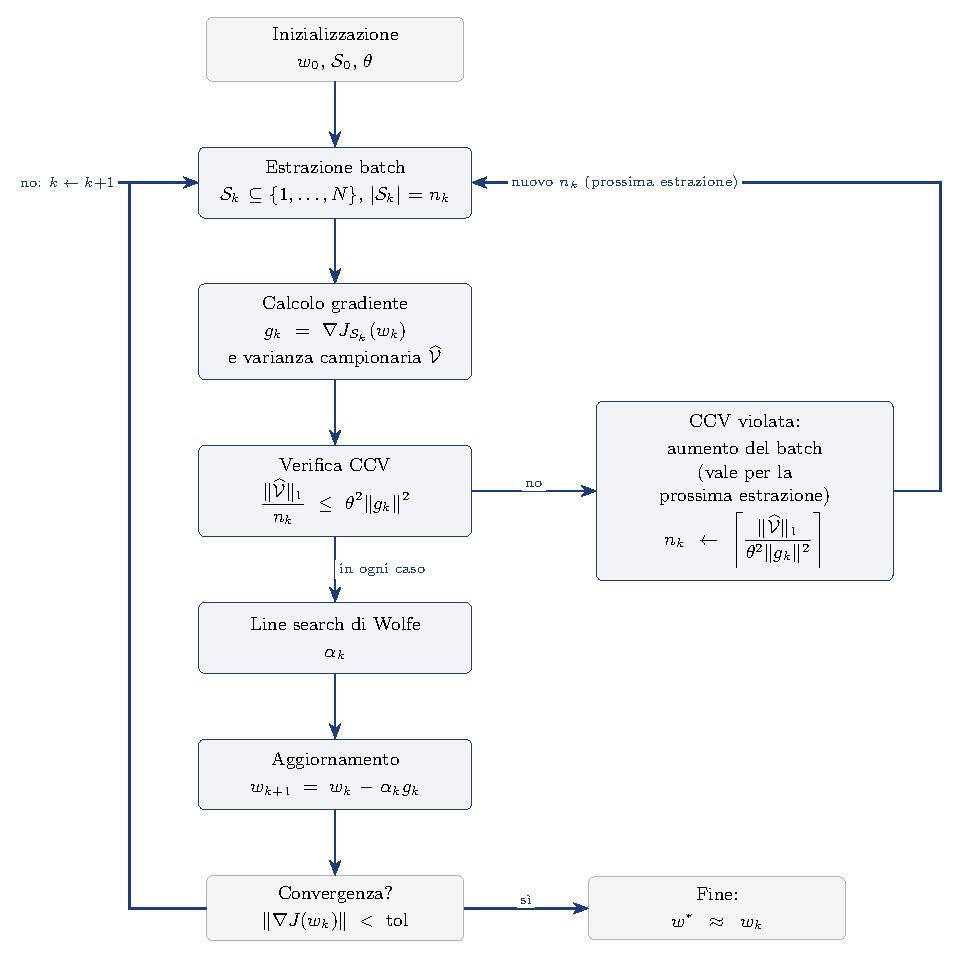
\includegraphics[height=0.67\paperheight]{schema_dynamic_gd.pdf}\\[0.2cm]
    {\small\color{grigio} Flusso CCV: se la varianza campionaria è troppo
      grande rispetto a $\theta^2\|g_k\|^2$, $n_k$ cresce e si ricampiona;
      altrimenti line search di Wolfe e aggiornamento.}
  \end{center}
\end{frame}

% =====================================================================
% SLIDE 15 — Newton-CG: struttura del metodo (due campioni)
% =====================================================================
\begin{frame}{Newton-CG: struttura del metodo (eq.~5.31--5.32)}
  \small
  \setlength{\abovedisplayskip}{1pt}
  \setlength{\belowdisplayskip}{1pt}
  \setlength{\abovedisplayshortskip}{1pt}
  \setlength{\belowdisplayshortskip}{1pt}
  \begin{itemize}\setlength{\itemsep}{1pt}
    \item Due campioni a ogni iterazione: $\mathcal{S}_k$ per il
      \textbf{gradiente} (campionamento dinamico con CCV) e
      $\mathcal{H}_k\subset\mathcal{S}_k$ per l'\textbf{Hessiana}, con
      $|\mathcal{H}_k|\ll|\mathcal{S}_k|$ (prodotti Hessiana-vettore
      economici).
    \item La direzione di ricerca $d_k$ è la soluzione approssimata del
      sistema (Hessian-free: la matrice non è mai costruita)
      \[
        \nabla^2 J_{\mathcal{H}_k}(w_k)\,d=-\nabla J_{\mathcal{S}_k}(w_k).
      \]
    \item Rapporto di sottocampionamento fissato a priori e costante;
      quando $\mathcal{S}_k$ cresce (CCV) cresce in proporzione anche
      $\mathcal{H}_k$:
      \[
        R=\frac{|\mathcal{H}_k|}{|\mathcal{S}_k|}<1,
        \qquad
        |\mathcal{H}_k|=\bigl\lceil R\,|\mathcal{S}_k|\bigr\rceil .
      \]
      Linea guida: il costo dei prodotti Hessiana-vettore nel CG non deve
      superare quello di $\nabla J_{\mathcal{S}_k}(w_k)$.
  \end{itemize}
  \fonte{Dalla tesi --- Sez.~5.2, eq.~5.31--5.32}
\end{frame}

% =====================================================================
% SLIDE 16 — Newton-CG: non serve un residuo più piccolo dell'errore
%            di Hessiana
% =====================================================================
\begin{frame}{Newton-CG: non serve un residuo più piccolo dell'errore di Hessiana}
  \footnotesize
  \setlength{\abovedisplayskip}{1pt}
  \setlength{\belowdisplayskip}{1pt}
  \setlength{\abovedisplayshortskip}{1pt}
  \setlength{\belowdisplayshortskip}{1pt}
  \begin{itemize}\setlength{\itemsep}{0pt}
    \item Il CG risolve in modo \textbf{approssimato} il sistema di Newton
      (eq.~5.31), gradiente su $\mathcal{S}_k$ e Hessiana su $\mathcal{H}_k$;
      il suo \textbf{residuo} è (eq.~5.33):
      \[
        r_k=\nabla^2J_{\mathcal{H}_k}(w_k)\,d+\nabla J_{\mathcal{S}_k}(w_k),
      \]
    \item L'Hessiana è quindi \textbf{approssimata}: il residuo del sistema
      che userebbe il campione grande $\mathcal{S}_k$ per gradiente ed
      Hessiana si scompone in
      \[
        \nabla^2J_{\mathcal{S}_k}(w_k)d+\nabla J_{\mathcal{S}_k}(w_k)
        =\underbrace{r_k}_{\text{residuo del CG}}
        +\underbrace{\Delta_{\mathcal{H}_k}(w_k;d)}_{\text{errore di Hessiana}},
      \]
      dove
      $\Delta_{\mathcal{H}_k}(w_k;d)=\bigl[\nabla^2J_{\mathcal{S}_k}(w_k)
      -\nabla^2J_{\mathcal{H}_k}(w_k)\bigr]d$ è \textbf{costante durante il
      CG} e \textbf{non eliminabile} (il campione $\mathcal{H}_k$ è fissato).
    \item Poiché $\Delta_{\mathcal{H}_k}$ non si può eliminare, \emph{non
      serve} ridurre $r_k$ fino a zero: \textbf{basta fermarlo quando è
      confrontabile con $\Delta_{\mathcal{H}_k}$}; oltre, le iterazioni del CG
      sono \emph{tempo sprecato}.
    \item \kw{Perché non è calcolabile?} Conterrebbe la media su tutto
      $\mathcal{S}_k$ dei prodotti Hessiana--vettore
      $\nabla^2\ell(w_k;i)d$: costerebbe quanto l'Hessiana piena e
      \textbf{vanificherebbe} il sottocampionamento di $\mathcal{H}_k$. Come
      per l'errore $e_k$ del gradiente: la si stima con la \textbf{varianza
      campionaria} dei prodotti Hessiana--vettore su $\mathcal{H}_k$.
  \end{itemize}
  \fonte{Dalla tesi --- Sez.~5.2, eq.~5.31 e 5.33--5.34 e discussione del criterio}
\end{frame}

% =====================================================================
% SLIDE 17 — Newton-CG: come si stima l'errore di Hessiana
% =====================================================================
\begin{frame}{Newton-CG: come si stima l'errore di Hessiana (eq.~5.35)}
  \small
  \setlength{\abovedisplayskip}{3pt}
  \setlength{\belowdisplayskip}{3pt}
  \setlength{\abovedisplayshortskip}{3pt}
  \setlength{\belowdisplayshortskip}{3pt}
  \begin{itemize}\setlength{\itemsep}{3pt}
    \item $\Delta_{\mathcal{H}_k}(w_k;d)$ \textbf{non è calcolabile}
      (servirebbe il prodotto Hessiana--vettore su tutto $\mathcal{S}_k$):
      come per l'errore del gradiente, se ne stima il valore atteso con la
      \textbf{varianza campionaria dei prodotti Hessiana--vettore} su
      $\mathcal{H}_k$ (campionamento senza reinserimento: fattore
      $(|\mathcal{S}_k|-|\mathcal{H}_k|)/(|\mathcal{S}_k|-1)\approx1$ perché
      $|\mathcal{H}_k|\ll|\mathcal{S}_k|$):
      \[
        \mathbb{E}\bigl[\|\Delta_{\mathcal{H}_k}(w_k;d)\|_2^2\bigr]
        \approx\frac{\bigl\|\mathrm{Var}_{i\in\mathcal{H}_k}
          \bigl(\nabla^2\ell(w_k;i)\,d\bigr)\bigr\|_1}{|\mathcal{H}_k|}.
      \]
      Come per il gradiente: è la varianza della \emph{media} su
      $\mathcal{H}_k$ (la dispersione dei singoli prodotti divisa per
      $|\mathcal{H}_k|$).
    \item La stima vale per una direzione generica $d$: nel CG andrebbe
      rivalutata a ogni iterazione interna $j$, sulla direzione corrente
      $d_j$. Ricalcolare la varianza campionaria a ogni passo è però
      costoso: la prossima slide mostra come si evita.
  \end{itemize}
  \fonte{Dalla tesi --- Sez.~5.2, eq.~5.35}
\end{frame}

% =====================================================================
% SLIDE 18 — Omogeneità di grado 2 e un solo calcolo
% =====================================================================
\begin{frame}{Newton-CG: omogeneità di grado 2 e un solo calcolo (eq.~5.36--5.38)}
  \footnotesize
  \setlength{\abovedisplayskip}{1pt}
  \setlength{\belowdisplayskip}{1pt}
  \setlength{\abovedisplayshortskip}{1pt}
  \setlength{\belowdisplayshortskip}{1pt}
  \begin{itemize}\setlength{\itemsep}{0pt}
    \item Su un campione fissato, la varianza dei prodotti
      Hessiana--vettore è una \textbf{forma quadratica} in $d$:
      $\mathrm{Var}\bigl(\nabla^2\ell(w_k;i)d\bigr)
      =d^T\Sigma_{\mathcal{H}_k}d$ ($\Sigma_{\mathcal{H}_k}$ covarianza
      campionaria sdp; la relazione vale componente per componente). Vale
      quindi l'\textbf{omogeneità di grado 2}
      \[
        \mathrm{Var}_{i\in\mathcal{H}_k}\bigl(\nabla^2\ell(w_k;i)(\lambda d)\bigr)
        =\lambda^2\,\mathrm{Var}_{i\in\mathcal{H}_k}\bigl(\nabla^2\ell(w_k;i)d\bigr).
      \]
    \item \textbf{Un solo calcolo.} Per non ricalcolare la varianza a ogni
      iterazione del CG (costo elevato), la si calcola \textbf{una sola
      volta} sulla prima direzione $p_0=-g_k$,
      \[
        \alpha:=\frac{\bigl\|\mathrm{Var}_{i\in\mathcal{H}_k}\bigl(\nabla^2
        \ell(w_k;i)\,p_0\bigr)\bigr\|_1}{\|p_0\|_2^2}
        =\frac{\bigl\|p_0^T\Sigma_{\mathcal{H}_k}p_0\bigr\|_1}{\|p_0\|_2^2},
      \]
      e per ogni $d_j$ si usa
      $\bigl\|\mathrm{Var}_{i\in\mathcal{H}_k}\bigl(\nabla^2\ell(w_k;i)d_j\bigr)
      \bigr\|_1\approx\alpha\,\|d_j\|_2^2$.
    \item \textbf{Approssimazione.} La varianza effettiva di $d_j$ è
      $\|d_j^T\Sigma_{\mathcal{H}_k}d_j\|_1$, non $\alpha\|d_j\|^2$: $\alpha$
      è la media pesata degli autovalori di $\Sigma_{\mathcal{H}_k}$
      ($\lambda_{\min}\le\alpha\le\lambda_{\max}$) e usarla su tutte le
      direzioni è lecito se la forma quadratica è sufficientemente
      \emph{ben condizionata} (dipendenza angolare trascurabile).
    \item Dalla (5.35), la soglia per il test di arresto del CG è
      $\gamma:=\alpha/|\mathcal{H}_k|$ e $\Psi(d):=\gamma\|d\|_2^2$: per ogni
      $d_j$, $\Psi(d_j)\approx\mathbb{E}\|\Delta_{\mathcal{H}_k}(w_k;d_j)\|_2^2$
      \textbf{cresce con $\|d_j\|^2$} (prossima slide: criterio di arresto).
  \end{itemize}
  \fonte{Dalla tesi --- Sez.~5.2, eq.~5.36--5.38}
\end{frame}

% =====================================================================
% SLIDE 19 — Newton-CG: criterio di arresto adattivo del CG
% =====================================================================
\begin{frame}{Newton-CG: criterio di arresto adattivo del CG (eq.~5.39)}
  \small
  \setlength{\abovedisplayskip}{3pt}
  \setlength{\belowdisplayskip}{3pt}
  \setlength{\abovedisplayshortskip}{3pt}
  \setlength{\belowdisplayshortskip}{3pt}
  \begin{itemize}\setlength{\itemsep}{3pt}
    \item A ogni iterazione interna $j$ del CG si confronta il residuo
      $r_{j+1}$ con la stima $\Psi(d_j)$ dell'errore di Hessiana:
      \[
        \|r_{j+1}\|_2^2\;\le\;\Psi(d_j)=\gamma\,\|d_j\|_2^2.
      \]
      Se la condizione è verificata il CG \textbf{termina} e si accetta la
      direzione $d_{j+1}$; altrimenti si prosegue con l'iterazione
      successiva.
    \item È un criterio \emph{automatico}: $\gamma$ è fissata dai dati
      all'inizio del CG e la soglia $\Psi(d_j)$ si aggiorna a ogni iterazione
      con la sola $\|d_j\|_2^2$ e nessuna tolleranza da scegliere a priori.
    \item \kw{Perché è adattivo.}
      \begin{itemize}\setlength{\itemsep}{1pt}
        \item evita calcoli inutili quando l'approssimazione dell'Hessiana è
          limitata dal campione $\mathcal{H}_k$;
        \item $\Psi\propto\|r_0\|^2$: la soglia segue la \emph{distanza dal
          minimo};
        \item $\Psi$ cresce con $\|d_j\|^2$: ferma il CG prima che la
          direzione diventi eccessivamente grande (stabilità numerica).
      \end{itemize}
  \end{itemize}
  \fonte{Dalla tesi --- Sez.~5.2, eq.~5.39 e discussione del criterio}
\end{frame}

% =====================================================================
% SLIDE 20 — Schema: Newton-CG (Fig. 5.2)
% =====================================================================
\begin{frame}{Schema: Newton-CG (Fig.~5.2)}
  \begin{center}
    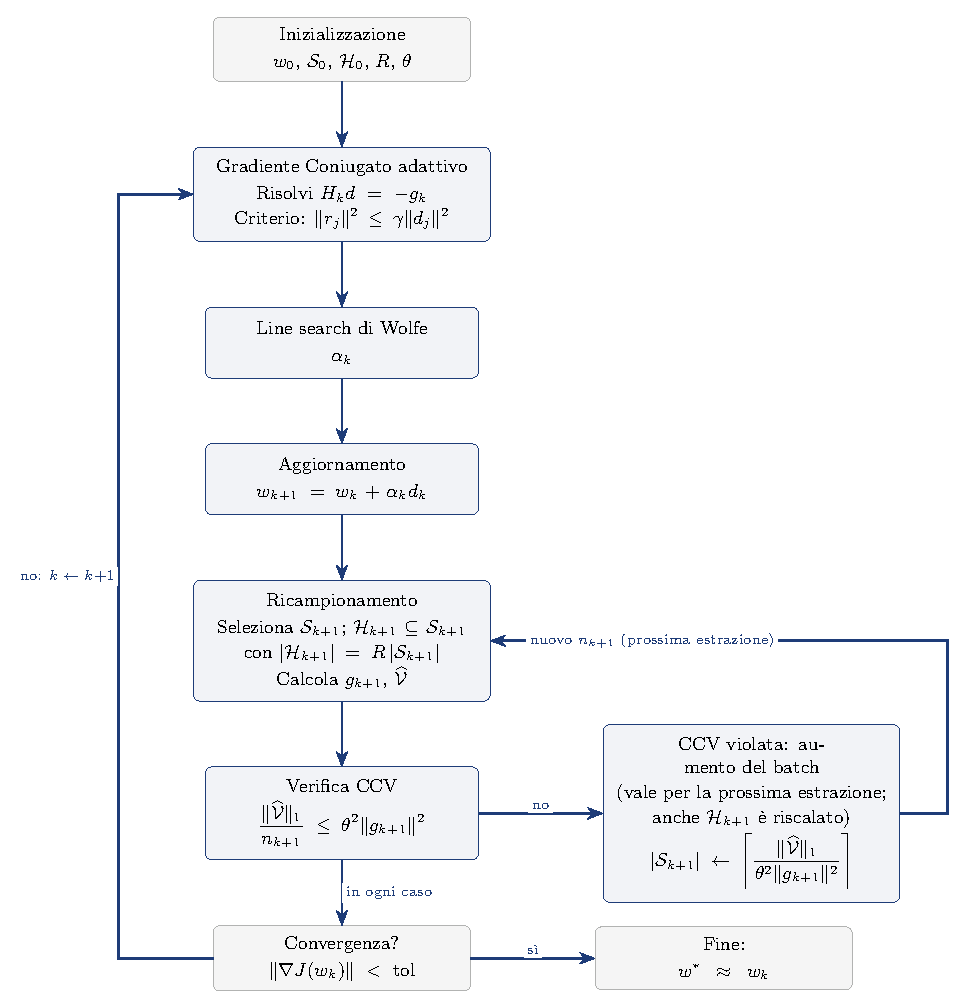
\includegraphics[height=0.67\paperheight]{schema_newton_cg.pdf}\\[0.2cm]
    {\small\color{grigio} Hessiana sottocampionata con $|\mathcal{H}|=R\,|\mathcal{S}|$;
      il CG interno è Hessian-free e si ferma con un criterio adattivo basato
      sulla varianza dei prodotti Hessiana-vettore.}
  \end{center}
\end{frame}

% =====================================================================
% SLIDE 21 — Newton-CG L1: il gradiente generalizzato di F=J+nu||w||_1
% =====================================================================
\begin{frame}{Newton-CG $L_1$: il gradiente generalizzato di $F=J+\nu\|w\|_1$}
  \footnotesize
  \setlength{\abovedisplayskip}{2pt}
  \setlength{\belowdisplayskip}{2pt}
  \setlength{\abovedisplayshortskip}{2pt}
  \setlength{\belowdisplayshortskip}{2pt}
  \begin{itemize}\setlength{\itemsep}{2pt}
    \item $F(w)=J(w)+\nu\sum_{i=1}^{m}|w_i|$: parte liscia $J$ + parte non
      liscia $\nu\sum_i|w_i|$. La somma si decompone per componente
      $\Rightarrow$ il gradiente generalizzato si calcola coordinata per
      coordinata: per la $i$-esima servono
      \begin{enumerate}\setlength{\itemsep}{1pt}
        \item la derivata parziale della parte liscia:
          $\partial J(w)/\partial w_i$;
        \item il subgradiente di $\nu|w_i|$:
          $\partial(\nu|w_i|)=\{+\nu\}$ se $w_i>0$, $\{-\nu\}$ se $w_i<0$,
          $[-\nu,+\nu]$ se $w_i=0$.
      \end{enumerate}
    \item Quindi, per ogni componente,
      \[
        [\widetilde{\nabla}F(w)]_i
        =\underbrace{\frac{\partial J(w)}{\partial w_i}}_{\text{gradiente di }J}
        +\underbrace{g_i}_{\text{subgradiente di }\nu|w_i|},\qquad
        g_i\in\begin{cases}
          \{+\nu\}, & w_i>0,\\
          \{-\nu\}, & w_i<0,\\
          [-\nu,+\nu], & w_i=0.
        \end{cases}
      \]
    \item Quando $w_i=0$ c'è libertà su $g_i\in[-\nu,+\nu]$; la scelta è fatta
      in modo che in $w^*$ valga $\widetilde{\nabla}F(w^*)=0$. Posto
      $d_i:=\partial J(w)/\partial w_i$ (così
      $[\widetilde{\nabla}F]_i=d_i+g_i$), si prende
      $g_i=\arg\min_{g\in[-\nu,\nu]}|d_i+g|$: il subgradiente che rende
      $d_i+g_i$ il più vicino possibile a zero (zero se possibile), così
      $w_i=0$ è riconosciuto come vero minimo quando lo è. Ne derivano i tre
      casi:
      \begin{itemize}\setlength{\itemsep}{1pt}
        \item $d_i<-\nu\;\Rightarrow\;g_i=+\nu\;\Rightarrow\;
          [\widetilde{\nabla}F]_i<0$ ($w_i$ cresce);
        \item $-\nu\le d_i\le+\nu\;\Rightarrow\;g_i=-d_i\;\Rightarrow\;
          [\widetilde{\nabla}F]_i=0$ ($w_i=0$ stazionario);
        \item $d_i>+\nu\;\Rightarrow\;g_i=-\nu\;\Rightarrow\;
          [\widetilde{\nabla}F]_i>0$ ($w_i$ decresce).
      \end{itemize}
  \end{itemize}
  \fonte{Dalla tesi --- Sez.~5.3, ``Il gradiente generalizzato'' (eq.~5.43)}
\end{frame}

% =====================================================================
% SLIDE 22 — Newton-CG L1: z_k, active set e faccia ortante (eq. 5.43-5.46)
% =====================================================================
\begin{frame}{Newton-CG $L_1$: $z_k$, active set e faccia ortante}
  \footnotesize
  \setlength{\abovedisplayskip}{2pt}
  \setlength{\belowdisplayskip}{2pt}
  \setlength{\abovedisplayshortskip}{2pt}
  \setlength{\belowdisplayshortskip}{2pt}
  \begin{itemize}\setlength{\itemsep}{1pt}
    \item $F=J+\nu\|w\|_1$ non è differenziabile dove $w_i=0$: lì si sceglie
      $g_i$ (slide precedente) e la decisione se \emph{liberare} $w_i$ o
      \emph{attivarla} (tenerla a zero, per la sparsità) è codificata da
      $z_k\in\{-1,0,+1\}^m$ (eq.~5.44):
      \[
        z_k^i=\begin{cases}
          +1 & w_k^i>0 \ \text{oppure}\ \bigl(w_k^i=0 \text{ e }
          \partial J_{\mathcal{S}_k}/\partial w_i<-\nu\bigr)\\[2pt]
          -1 & w_k^i<0 \ \text{oppure}\ \bigl(w_k^i=0 \text{ e }
          \partial J_{\mathcal{S}_k}/\partial w_i>\nu\bigr)\\[2pt]
          0 & \text{altrimenti}
        \end{cases}
      \]
    \item \textbf{Active set} (eq.~5.46): $\mathcal{A}_k=\{i:z_k^i=0\}$ sono
      le variabili tenute a zero durante la minimizzazione; le altre sono
      \emph{libere}.
    \item $z_k$ definisce la \textbf{faccia ortante} (eq.~5.45)
      $\Omega_k=\{d:\operatorname{sign}(d^i)=\operatorname{sign}(z_k^i)\}$,
      dove $\|w\|_1$ è lineare e il gradiente generalizzato è
      $\widetilde{\nabla}F_{\mathcal{S}_k}(w_k)=\nabla J_{\mathcal{S}_k}(w_k)
      +\nu z_k$ (eq.~5.43); su $\Omega_k$ si minimizza il modello quadratico
      ristretto alle variabili libere.
  \end{itemize}
  \fonte{Dalla tesi --- Sez.~5.3, eq.~5.43--5.47}
\end{frame}


% =====================================================================
% SLIDE 23 — Newton-CG L1: ricerca lineare proiettata (eq. 5.49-5.50)
% =====================================================================
\begin{frame}{Newton-CG $L_1$: la ricerca lineare proiettata}
  \footnotesize
  \setlength{\abovedisplayskip}{2pt}
  \setlength{\belowdisplayskip}{2pt}
  \setlength{\abovedisplayshortskip}{2pt}
  \setlength{\belowdisplayshortskip}{2pt}
  \begin{itemize}\setlength{\itemsep}{1pt}
    \item Il candidato $w_k+\alpha_k d_k$ può \textbf{uscire dalla faccia}
      $\Omega_k$: una variabile attiva lascerebbe lo zero, una libera
      attraverserebbe l'angolo della $L_1$. Si proietta su $\Omega_k$
      (eq.~5.49):
      \[
        P(w_i)=\begin{cases}
          w_i & \operatorname{sign}(w_i)=\operatorname{sign}(z_k^i)\\
          0 & \text{altrimenti}
        \end{cases}
      \]
      La proiezione $P(\cdot)$ azzera le componenti con segno non coerente
      con $z_k$.
    \item Il passo è scelto con \textbf{Armijo su $F$} (eq.~5.50): $\alpha_k$
      è il più grande valore in $\{1,\tfrac12,\tfrac14,\dots\}$ tale che
      \[
        F_{\mathcal{S}_k}\bigl(P[w_k+\alpha_k d_k]\bigr)\;\le\;
        F_{\mathcal{S}_k}(w_k)+\sigma\,\widetilde{\nabla}F_{\mathcal{S}_k}
        (w_k)^T\bigl(P[w_k+\alpha_k d_k]-w_k\bigr),\qquad \sigma\in(0,1).
      \]
    \item Aggiornamento: $w_{k+1}=P[w_k+\alpha_k d_k]$; le variabili attive
      restano a zero $\Rightarrow$ soluzione sparsa.
  \end{itemize}
  \fonte{Dalla tesi --- Sez.~5.3, eq.~5.49--5.50}
\end{frame}


% =====================================================================
% SLIDE 24 — Schema: Newton-CG L1 (Fig. 5.5)
% =====================================================================
\begin{frame}{Schema: Newton-CG $L_1$ (Fig.~5.5)}
  \begin{center}
    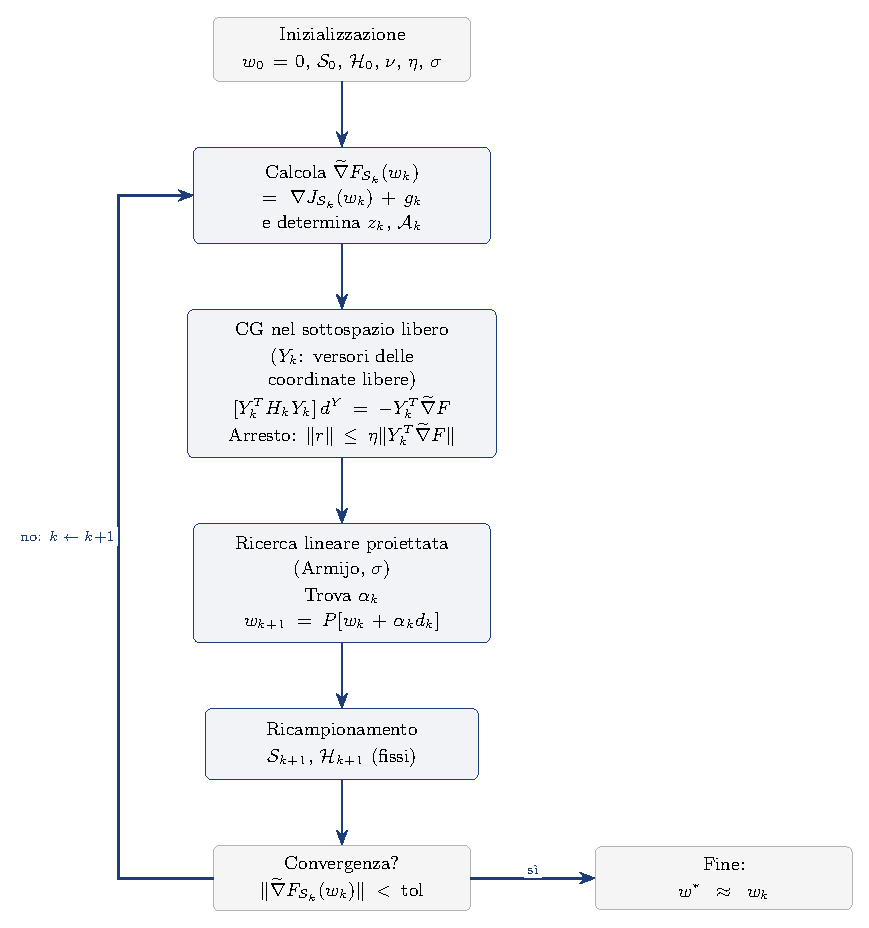
\includegraphics[height=0.67\paperheight]{schema_newton_l1.pdf}\\[0.2cm]
    {\small\color{grigio} Gradiente generalizzato per la $L_1$: identificazione
      dell'active set e line search proiettata mantengono a zero le variabili
      giuste, producendo soluzioni sparse.}
  \end{center}
\end{frame}

% =====================================================================
% SLIDE 25 — Il passo di Barzilai--Borwein (1/2): relazione secante e passo
% =====================================================================
\begin{frame}{Il passo di Barzilai--Borwein (1/2) --- relazione secante (eq.~5.52--5.54)}
  \small
  \setlength{\abovedisplayskip}{2pt}
  \setlength{\belowdisplayskip}{2pt}
  \setlength{\abovedisplayshortskip}{2pt}
  \setlength{\belowdisplayshortskip}{2pt}
  \begin{itemize}\setlength{\itemsep}{2pt}
    \item BB-CCV sostituisce il passo \emph{fisso} del Dynamic GD con un passo
      \textbf{adattivo} che stima la curvatura di $J$ lungo la direzione
      percorsa usando \textbf{solo gradienti già calcolati}: nessuna Hessiana.
    \item Tra due iterate consecutive, $w_{k+1}=w_k+\Delta w_k$, lo sviluppo al
      primo ordine del gradiente $g=\nabla J$ attorno a $w_k$ è
      \[
        g(w_{k+1})\approx g(w_k)+\nabla^2J(w_k)\,\Delta w_k .
      \]
    \item Posto $s_k:=w_{k+1}-w_k$ (spostamento) e $y_k:=g(w_{k+1})-g(w_k)$
      (variazione del gradiente), si ha la \textbf{relazione secante}
      \[
        y_k\approx\nabla^2J(w_k)\,s_k .
      \]
    \item I metodi quasi-Newton approssimano l'Hessiana con $B_{k+1}$
      imponendo $B_{k+1}s_k=y_k$: è il punto di partenza del passo BB
      (prossima slide).
  \end{itemize}
  \fonte{Dalla tesi --- Sez.~5.4, eq.~5.52--5.54}
\end{frame}

% =====================================================================
% SLIDE 26 — Barzilai--Borwein (2/2): le due formule e la salvaguardia
% =====================================================================
\begin{frame}{Il passo di Barzilai--Borwein (2/2) --- minimi quadrati e salvaguardia (eq.~5.55--5.56)}
  \small
  \setlength{\abovedisplayskip}{2pt}
  \setlength{\belowdisplayskip}{2pt}
  \setlength{\abovedisplayshortskip}{2pt}
  \setlength{\belowdisplayshortskip}{2pt}
  \begin{itemize}\setlength{\itemsep}{2pt}
    \item BB spinge il quasi-Newton all'estremo: $B_{k+1}=\alpha^{-1}I$ (passo
      \textbf{scalare}); la secante diventa $\alpha^{-1}s\approx y$, un
      sistema di $n$ equazioni in un'incognita risolto \textbf{ai minimi
      quadrati}. Le due formule classiche:
      \[
        \alpha_k^{(1)}=\frac{s_k^\top y_k}{y_k^\top y_k}
        \quad(\min\|\alpha y-s\|^2),\qquad
        \alpha_k^{(2)}=\frac{s_k^\top s_k}{s_k^\top y_k}
        \quad(\min\|\alpha^{-1}s-y\|^2).
      \]
    \item BB-CCV usa la \textbf{seconda}, più \emph{aggressiva}: passi più
      grandi dove il gradiente cambia poco (direzione piatta), più piccoli
      dove cambia molto.
    \item \textbf{Rischio:} se $s^\top y\approx0$ (spostamento e variazione del
      gradiente quasi perpendicolari) il passo esplode; la \textbf{salvaguardia}
      $\mathrm{clip}\!\bigl(s^\top s/s^\top y,\ \alpha/20,\ 5\alpha\bigr)$ lo
      tiene in $[\alpha/20,\,5\alpha]$.
    \item Su $J$ quadratiche ($y=As$ esatta, $A$ definita positiva) il passo è
      \textbf{ottimale}: poche iterazioni. Su $J$ generali la secante è solo
      locale e $s^\top y$ può diventare $\le0$: stabilizzano salvaguardia e
      line search di Armijo.
  \end{itemize}
  \fonte{Dalla tesi --- Sez.~5.4, eq.~5.55--5.56 e salvaguardia clip}
\end{frame}

% =====================================================================
% SLIDE 27 — Schema: BB-CCV (Fig. 5.6)
% =====================================================================
\begin{frame}{Schema: BB-CCV (Fig.~5.6)}
  \begin{center}
    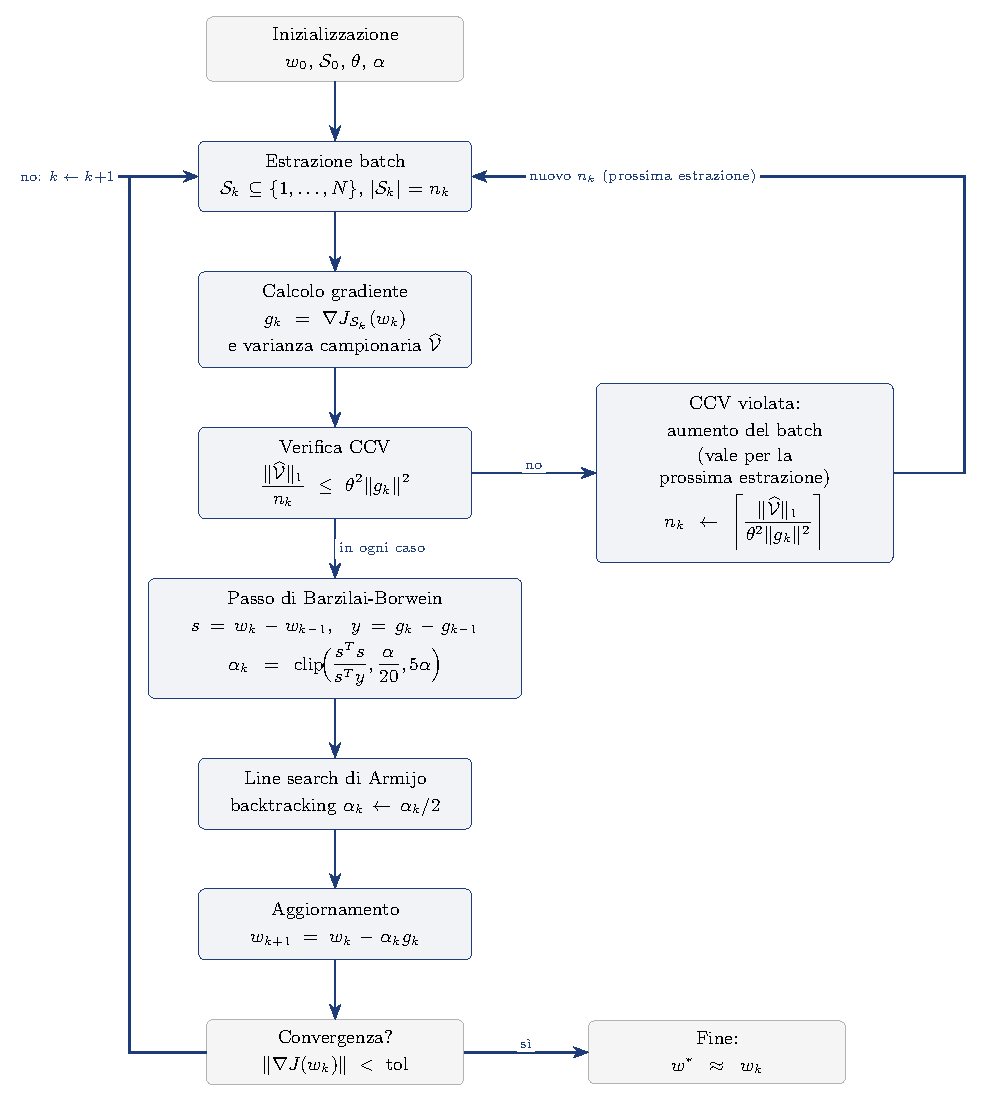
\includegraphics[height=0.67\paperheight]{schema_bbccv.pdf}\\[0.2cm]
    {\small\color{grigio} Gradiente dinamico con passo Barzilai--Borwein
      (line search di Armijo): la CCV regola la dimensione del campione
      mentre il passo adatta la lunghezza dello spostamento.}
  \end{center}
\end{frame}

% =====================================================================
% SLIDE 28 — App web interattiva
% =====================================================================
\begin{frame}{App web interattiva: esperimenti nel browser}
  \begin{itemize}
    \item \texttt{visualizzazione.html}: singolo file, Pyodide + Plotly,
      nessuna installazione o server.
    \item Codice Python dei quattro algoritmi visibile e modificabile nel
      browser; preset quadratici + dataset sintetico ``centrato''
      ($\widehat J_N = J$).
    \item Percorso 3D/2D su $J(w)$, metriche in tempo reale, pannelli
      ``Analisi'' e ``Test batch'' (per riprodurre le tabelle della tesi).
    \item Permette di osservare la dinamica del batch ($n_k$ vs $k$) e
      l'effetto del parametro $\theta$ sulla soglia CCV.
  \end{itemize}
\end{frame}
% =====================================================================
% SLIDE 29 — Le funzioni test: espressioni usate negli esperimenti
% =====================================================================
\begin{frame}{Le funzioni test: espressioni usate negli esperimenti}
  \footnotesize
  \setlength{\abovedisplayskip}{2pt}
  \setlength{\belowdisplayskip}{2pt}
  \setlength{\abovedisplayshortskip}{2pt}
  \setlength{\belowdisplayshortskip}{2pt}
  \begin{itemize}\setlength{\itemsep}{1pt}
    \item \textbf{Ben condizionata} ($\kappa\approx1.1$):
      $J(w)=(w_1-1)^2+(w_2+2)^2+0.1\,w_1w_2$
    \item \textbf{Mal condizionata} ($\kappa\approx20$):
      $J(w)=20\,(w_1-1)^2+(w_2+2)^2$
    \item \textbf{Molto mal condizionata} ($\kappa\approx100$):
      $J(w)=100\,(w_1-1)^2+(w_2+2)^2$
    \item \textbf{Termine incrociato} ($\kappa\approx1.67$):
      $J(w)=(w_1-1)^2+(w_2+2)^2+0.5\,(w_1-1)(w_2+2)$
    \item \textbf{Funzione di Rosenbrock} (non quadratica, $c{=}100$):
      \[
        J(w)=\frac{1}{N}\sum_{i=1}^N\Bigl[(w_1-a_i)^2+
        100\bigl((w_2-b_i)-(w_1-a_i)^2\bigr)^2\Bigr],
      \]
      con $a_i,b_i$ stocastici centrati ($\sigma=0.2$, medie $1$ e $-2$),
      $N=200$, seed 42: $w_*\approx(1.06,-1.96)$.
    \item Minimo comune dei quattro problemi quadratici:
      $w_*=(1,-2)$ (dataset centrato, $\widehat J_N=J$).
  \end{itemize}
  \fonte{Dalla tesi --- Sez.~6.1 (Setup Sperimentale)}
\end{frame}

% =====================================================================
% SLIDE 30 — Il dataset sintetico ``centrato’’: J(w) vs hat J_N(w)
% =====================================================================
\begin{frame}{Il dataset sintetico ``centrato'': $J(w)$ vs $\widehat J_N(w)$}
  \small
  \setlength{\abovedisplayskip}{2pt}
  \setlength{\belowdisplayskip}{2pt}
  \setlength{\abovedisplayshortskip}{2pt}
  \setlength{\belowdisplayshortskip}{2pt}
  \begin{itemize}\setlength{\itemsep}{2pt}
    \item Nel codice la \textbf{superficie plottata} è la funzione obiettivo
      teorica $J(w)$ (preset della loss): serve per disegnare il grafico,
      calcolare il percorso e mostrare le metriche $J(w_k)$ e
      $\|\nabla J(w_k)\|$.
    \item L'algoritmo però \textbf{non minimizza} $J(w)$: usa un dataset
      sintetico di $N$ funzioni di perdita individuali
      $\ell(w;i)$, $i=1,\dots,N$, costruito \emph{perturbando i coefficienti}
      di $J(w)$; ogni $\ell(w;i)$ è il contributo del singolo esempio $i$.
    \item A ogni iterazione si estrae un batch $\mathcal S_k$ di dimensione
      $n_k$ e si calcola il \textbf{gradiente del batch}
      $g_k=\frac{1}{n_k}\sum_{i\in\mathcal S_k}\nabla\ell(w_k;i)$; la line
      search di Armijo usa la \textbf{loss del batch}
      $J_{\mathcal S_k}(w)=\frac{1}{n_k}\sum_{i\in\mathcal S_k}\ell(w;i)$.
      La media su tutti gli $N$ dati è
      $\widehat J_N(w)=\frac{1}{N}\sum_{i=1}^{N}\ell(w;i)$.
    \item \textbf{Dataset ``centrato'':} le medie campionarie dei coefficienti
      delle perturbazioni coincidono esattamente con i coefficienti di $J(w)$
      $\Rightarrow$ $\widehat J_N(w)=J(w)$ e
      $\nabla\widehat J_N(w)=\nabla J(w)$ per ogni $w$,
      \emph{indipendentemente da $N$} (si sottrae a ogni perturbazione la
      propria media campionaria).
    \item Quindi $J(w)$ è la funzione plottata, ma l'algoritmo minimizza
      $\widehat J_N(w)$ (o sue approssimazioni su batch); la loss campionaria
      totale $\widehat J_N(w)$ è usata per la \textbf{condizione di arresto}.
      Nel codice la coincidenza $\widehat J_N=J$ vale per ogni $N$
      \emph{esattamente}; in un problema reale solo nel limite $N\to\infty$.
  \end{itemize}
  \fonte{Dalla tesi --- Sez.~6.2 (Architettura Software), ``Costruzione del
    dataset sintetico centrato''}
\end{frame}



% =====================================================================
% SLIDE 31 — Setup e risultati numerici
% =====================================================================
\begin{frame}{Setup e risultati numerici}
  \footnotesize
  \begin{columns}[T]
    \begin{column}{0.38\textwidth}
      \begin{itemize}\setlength{\itemsep}{1pt}
        \item Setup: $N=200$, seed 42, $w_0=(2,-3)$, $\alpha=0.1$,
          $\theta=0.5$, $n_0=5$, 30 iterazioni, $\|\nabla J\|_2<10^{-6}$
          (Wolfe; Armijo per BB-CCV).
        \item Funzioni test (5): ben condizionata ($\kappa\approx1.1$), mal
          ($\kappa\approx20$), molto mal ($\kappa\approx100$), incrociato
          ($\kappa\approx1.67$) e \textbf{Funzione di Rosenbrock} (non
          quadratica, $c{=}100$); formule a slide~28.
        \item $n_k$ a ``scalini'': il batch cresce solo se la CCV è violata
          (Fig.~5.3).
        \item BB-CCV su $\kappa\approx100$: $1.0991\times10^{-14}$
          (precisione macchina, cella verde in tabella).
      \end{itemize}
    \end{column}
    \begin{column}{0.62\textwidth}
      \begin{center}
      {\color{black}\everymath{\color{black}}%
        \renewcommand{\arraystretch}{0.85}%
        \setlength{\tabcolsep}{2.5pt}%
        \arrayrulecolor{grigio}%
        \scriptsize
        \scalebox{0.52}{%
        \begin{tabular}{@{}lcccc@{}}
        \toprule
        \cellcolor{white}Problema & \cellcolor{white}Dynamic GD &
        \cellcolor{white}BB-CCV & \cellcolor{white}Newton-CG &
        \cellcolor{white}Newton-CG $L_1$\\
        \midrule
        \cellcolor{white}$\kappa\approx1.1$ & \colorcell{1.1895}{-1} &
        \colorcell{1.1662}{-1} & \colorcell{4.0264}{-1} &
        \colorcell{1.0167}{-1}\\
        \cellcolor{white}$\kappa\approx20$ & \colorcell{4.9050}{-2} &
        \colorcell{9.7195}{-5} & \colorcell{2.3463}{-1} &
        \colorcell{4.8802}{-1}\\
        \cellcolor{white}$\kappa\approx100$ & \colorcell{4.6668}{-1} &
        \colorcell{1.0991}{-14} & \colorcell{2.0969}{-1} &
        \colorcell{9.6954}{-1}\\
        \cellcolor{white}incrociato ($\kappa\approx1.67$) &
        \colorcell{9.4161}{-3} & \colorcell{6.1644}{-4} &
        \colorcell{3.5167}{-1} & \colorcell{2.0877}{-2}\\
        \cellcolor{white}Rosenbrock ($c{=}100$) & \colorcell{6.1354}{-4} &
        \colorcell{1.0645}{-1} & \colorcell{2.0625}{-1} &
        \colorcell{1.2525}{-1}\\
        \bottomrule
        \end{tabular}}}
        \par
      \end{center}
      \vspace{-0.05cm}
      {\scriptsize\color{grigio} $e_{30}$ = errore finale (base, seed~42),
        come in tesi\_finale (Tab.~riuso\_sintesi): sfondo su scala log,
        verde = minimo, rosso = massimo.}
    \end{column}
  \end{columns}
\end{frame}

% =====================================================================
% SLIDE 32 — Riuso del mini-batch (Sez. 6.5)
% =====================================================================
\begin{frame}{Riuso del mini-batch (Sez.~6.5)}
  \begin{columns}[T]
    \begin{column}{0.55\textwidth}
      \begin{itemize}
        \item Variante studiata nella tesi: riusare lo stesso campione per
          $M$ iterazioni consecutive (ricalcolando però il gradiente al punto
          corrente, non riusando i gradienti vecchi).
        \item La CCV fa da segnale di ``esaurimento'' del campione: quando
          non è più soddisfatta, $n_k$ cresce e si ricampiona.
        \item $M=\infty$: si tiene il campione finché la CCV vale; il costo
          per iterazione scende, ma il campione ``invecchia''.
        \item Effetti dipendenti dal metodo e dal condizionamento del
          problema: quantificati con le tabelle del Cap.~6.
      \end{itemize}
    \end{column}
    \begin{column}{0.45\textwidth}
      \begin{center}
        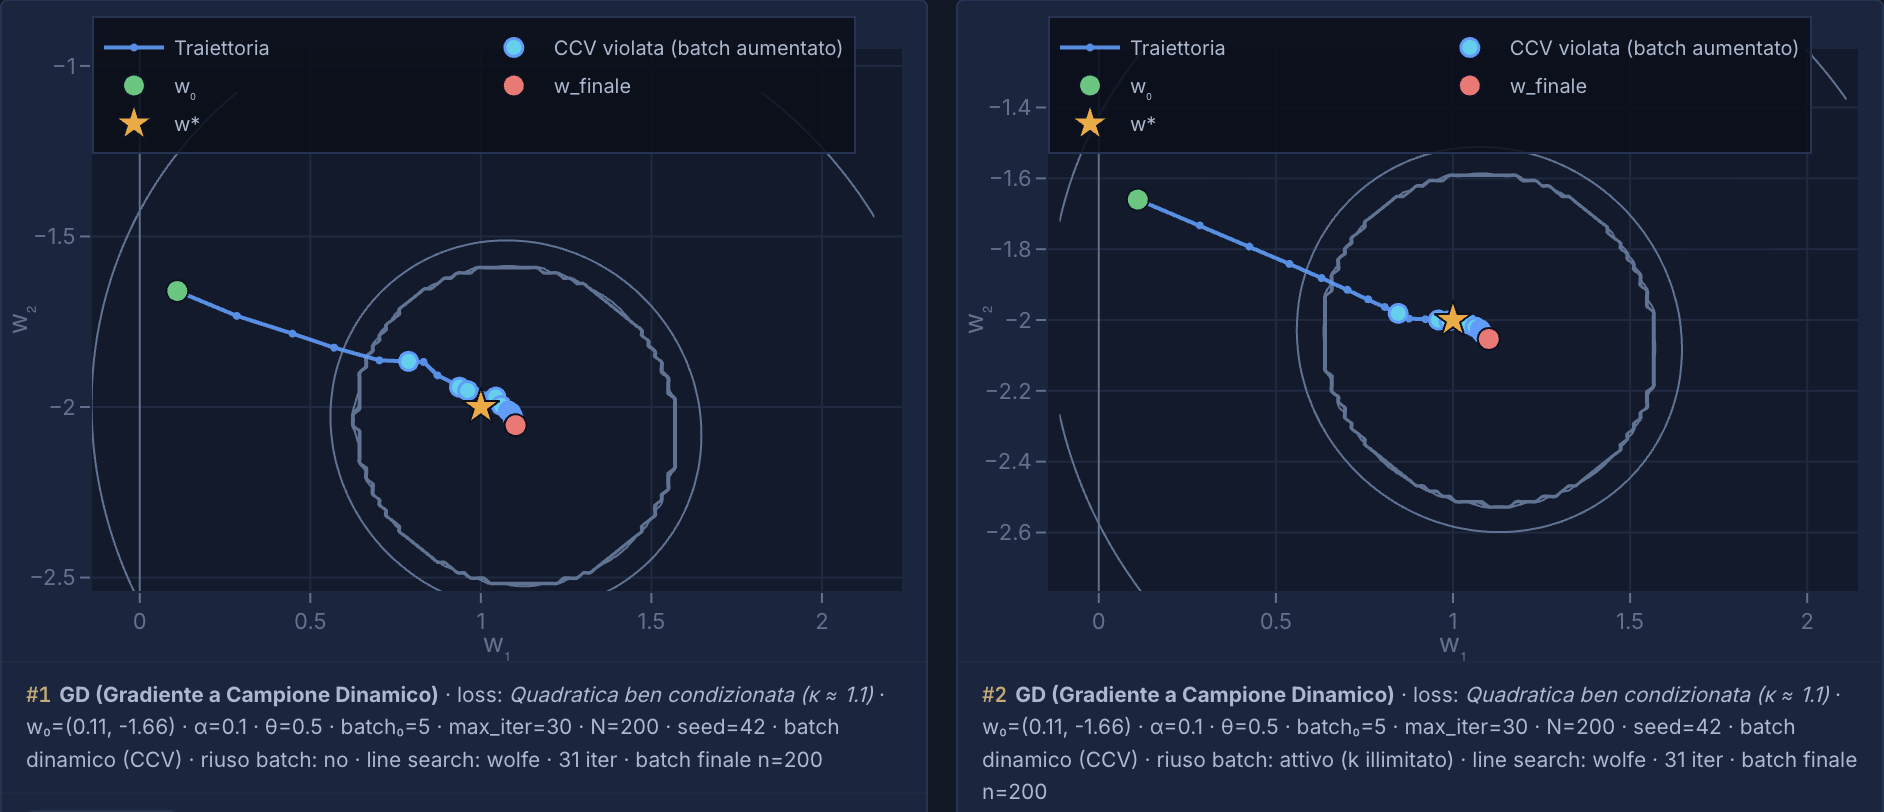
\includegraphics[width=\textwidth]{fig_riuso.png}\\[0.2cm]
        {\small\color{grigio} Traiettorie con riuso del batch}
      \end{center}
    \end{column}
  \end{columns}
\end{frame}

% =====================================================================
% SLIDE 33 — Cosa significa riusare il batch
% =====================================================================
\begin{frame}{Cosa significa riusare il batch}
  \small
  \setlength{\abovedisplayskip}{1pt}
  \setlength{\belowdisplayskip}{1pt}
  \setlength{\abovedisplayshortskip}{1pt}
  \setlength{\belowdisplayshortskip}{1pt}
  \begin{itemize}\setlength{\itemsep}{0pt}
    \item Riusare il batch = tenere \textbf{fissa solo la lista di indici}
      $\mathcal{S}_k$ per $M$ iterazioni; il gradiente è \textbf{ricalcolato
      al punto corrente} $w_k$ a ogni iterazione (non si riusa il gradiente
      né una ``direzione vecchia'').
    \item Sui \emph{ben condizionati} la traiettoria sembra ``dritta''
      perché $w^*_{\mathcal S}$ è vicino a $w^*$ in ogni direzione: i gradienti
      successivi puntano quasi allo stesso bersaglio.
    \item Sui \emph{mal condizionati} il minimo campionario $w^*_{\mathcal S}$
      è spostato lungo la direzione quasi piatta: il batch fisso ``tira''
      verso un bersaglio sbagliato (\textbf{bias sistematico}, Sez.~6.5.2),
      che la CCV \textbf{non} vede (misura la varianza interna, non il bias).
    \item \textbf{Primo ordine} (Dynamic GD, BB-CCV): $d_k=-g_k$ è sempre
      opposto al gradiente fresco (angolo $180^\circ$), la discesa sul batch è
      garantita: il rischio è solo la lenta \emph{deriva} verso $w^*_{\mathcal S}$.
    \item \textbf{Secondo ordine} (Newton-CG): con $\mathcal{H}_k$ fisso la
      curvatura ``invecchia'' mentre $w_k$ avanza; $d_k=-H_k^{-1}g_k$ può
      finire a $\approx90^\circ$ dalla vera discesa e la line search taglia il
      passo $\Rightarrow$ per questo serve lo stop adattivo (slide seguenti).
  \end{itemize}
  \fonte{Dalla tesi --- Sez.~6.5.2, ``Meccanismo: vantaggi e limiti del riuso''}
\end{frame}

% =====================================================================
% SLIDE 34 — Perché il riuso è critico sui mal condizionati (esempio κ)
% =====================================================================
\begin{frame}{Perché il riuso è critico sui mal condizionati: l'esempio $\kappa$}
  \small
  \setlength{\abovedisplayskip}{1pt}
  \setlength{\belowdisplayskip}{1pt}
  \setlength{\abovedisplayshortskip}{1pt}
  \setlength{\belowdisplayshortskip}{1pt}
  \textbf{Modello} (Sez.~6.5.2): $J(w)=\kappa w_1^2+w_2^2$ con $w^*=(0,0)$,
  $\ell(w;i)=\kappa(w_1+\varepsilon_1^{(i)})^2+(w_2+\varepsilon_2^{(i)})^2$
  con $\varepsilon^{(i)}\sim\mathcal N(0,0.04\,I)$. La media sugli $N$ esempi è
  $J(w)$, ma ogni loss è centrata in un punto diverso.
  \begin{itemize}\setlength{\itemsep}{2pt}
    \item \kw{Primo ordine ($d_k=-g_k$): deriva permanente.} Il gradiente
      sul batch punta al \emph{minimo campionario}
      $w^*_{\mathcal S}=(-\bar\varepsilon_1,-\bar\varepsilon_2)\ne w^*$:
      \[
        g_k=\nabla J_{\mathcal S_k}(w_k)=\bigl[2\kappa\,(w_1+\bar\varepsilon_1),\,
        2\,(w_2+\bar\varepsilon_2)\bigr]^{\!\top},\quad
        \bar\varepsilon_j=\frac{1}{n_k}\sum_{i\in\mathcal S_k}\varepsilon_j^{(i)}.
      \]
      Nella direzione quasi piatta $w_2$ il gradiente di $J$ è debolissimo:
      anche un piccolo $\bar\varepsilon_2\approx0.09$ ($n_k=5$) sposta di molto
      $w^*_{\mathcal S}$. Riusare lo stesso batch significa smettere di mediare
      il rumore: l'iterato \emph{deriva} verso $w^*_{\mathcal S}$, e la CCV non
      lo vede (misura la varianza interna, non il bias sistematico).
    \item \kw{Secondo ordine ($d_k=-H_k^{-1}g_k$): Hessiana obsoleta.}
      $H_k$ compensa il condizionamento: se è stata calcolata dove il batch è
      stato estratto ma $w_k$ si è spostato, applica una curvatura
      \emph{vecchia} (allunga il passo dove la funzione è diventata ripida,
      lo accorcia dove è diventata piatta). Con $\kappa$ grande $d_k$ può
      formare $\approx90^\circ$ con la vera discesa: la line search taglia il
      passo e il metodo si \emph{blocca} lontano dal minimo
      ($e_{30}\approx1.28$ con $M{=}\infty$ su $\kappa\approx100$).
  \end{itemize}
  \fonte{Dalla tesi --- Sez.~6.5.2, ``Meccanismo: vantaggi e limiti del riuso''}
\end{frame}

% =====================================================================
% SLIDE 35 -- Riuso del mini-batch: sintesi dei risultati (Tab.6.1)
% =====================================================================
\begin{frame}{Riuso del mini-batch: sintesi dei risultati (Tab.~6.1)}
  \footnotesize
  \begin{itemize}\setlength{\itemsep}{1.5pt}
\item \textbf{Aiuta}: ben condizionato ($\kappa\approx1.1$), termine incrociato, BB-CCV su $\kappa\approx20$ (fino a $\sim10^{-10}$).
\item \textbf{Peggiora}: BB-CCV su $\kappa\approx100$ (base già alla precisione macchina, $\sim10^{-14}$) e Dynamic GD/Newton-CG sui mal condizionati con $M{=}\infty$ (direzioni che invecchiano).
  \end{itemize}
  \vspace{0.05cm}
  \begin{center}
    {
      \renewcommand{\arraystretch}{0.92}
      \setlength{\tabcolsep}{3pt}
      \arrayrulecolor{grigio}
      \color{black}\everymath{\color{black}}
      \scalebox{0.42}{%
        \begin{tabular}{@{}lrrrrrrr@{}}
\toprule
\cellcolor{white}Metodo & \cellcolor{white}\emph{base} & \cellcolor{white}$M{=}\infty$ & \cellcolor{white}$M{=}10$ & \cellcolor{white}$M{=}5$ & \cellcolor{white}$M{=}3$ & \cellcolor{white}$M{=}2$ & \cellcolor{white}$M{=}1$\\
\midrule
\cellcolor{white}$\kappa\approx1.1$ - Dynamic GD& \colorcell{1.1895}{-1} & \colorcell{1.1739}{-1} $\blacktriangle$ & \colorcell{1.1739}{-1} $\blacktriangle$ & \colorcell{1.1920}{-1} $\blacktriangledown$ & \colorcell{1.1903}{-1} $\blacktriangledown$ & \colorcell{1.1777}{-1} $\blacktriangle$ & \colorcell{1.1895}{-1} $=$\\
\cellcolor{white}$\kappa\approx1.1$ - BB-CCV& \colorcell{1.1662}{-1} & \colorcell{1.1662}{-1} $\blacktriangle$ & \colorcell{1.1662}{-1} $\blacktriangle$ & \colorcell{1.1662}{-1} $\blacktriangle$ & \colorcell{1.1662}{-1} $\blacktriangle$ & \colorcell{1.1662}{-1} $\blacktriangle$ & \colorcell{1.1662}{-1} $=$\\
\cellcolor{white}$\kappa\approx1.1$ - Newton-CG& \colorcell{4.0264}{-1} & \colorcell{2.2230}{-1} $\blacktriangle$ & \colorcell{3.7373}{-1} $\blacktriangle$ & \colorcell{4.1553}{-1} $\blacktriangledown$ & \colorcell{3.2913}{-1} $\blacktriangle$ & \colorcell{2.6069}{-1} $\blacktriangle$ & \colorcell{3.0560}{-1} $\blacktriangle$\\
\cellcolor{white}$\kappa\approx1.1$ - Newton-CG $L_1$& \colorcell{1.0167}{-1} & \colorcell{8.1750}{-2} $\blacktriangle$ & \colorcell{9.2407}{-2} $\blacktriangle$ & \colorcell{1.0010}{-1} $\blacktriangle$ & \colorcell{1.0624}{-1} $\blacktriangledown$ & \colorcell{9.4078}{-2} $\blacktriangle$ & \colorcell{1.0028}{-1} $\blacktriangle$\\
\midrule
\cellcolor{white}$\kappa\approx20$ - Dynamic GD& \colorcell{4.9050}{-2} & \colorcell{1.0103}{-1} $\blacktriangledown$ & \colorcell{7.6020}{-2} $\blacktriangledown$ & \colorcell{4.7211}{-2} $\blacktriangle$ & \colorcell{1.1746}{-1} $\blacktriangledown$ & \colorcell{4.2898}{-2} $\blacktriangle$ & \colorcell{4.9050}{-2} $=$\\
\cellcolor{white}$\kappa\approx20$ - BB-CCV& \colorcell{9.7195}{-5} & \colorcell{9.5364}{-10} $\blacktriangle$ & \colorcell{9.5364}{-10} $\blacktriangle$ & \colorcell{2.6835}{-3} $\blacktriangledown$ & \colorcell{3.8422}{-8} $\blacktriangle$ & \colorcell{1.5436}{-10} $\blacktriangle$ & \colorcell{9.7195}{-5} $=$\\
\cellcolor{white}$\kappa\approx20$ - Newton-CG& \colorcell{2.3463}{-1} & \colorcell{1.2807}{0} $\blacktriangledown$ & \colorcell{9.4933}{-1} $\blacktriangledown$ & \colorcell{4.1051}{-1} $\blacktriangledown$ & \colorcell{3.3396}{-1} $\blacktriangledown$ & \colorcell{4.0617}{-1} $\blacktriangledown$ & \colorcell{1.6683}{-1} $\blacktriangle$\\
\cellcolor{white}$\kappa\approx20$ - Newton-CG $L_1$& \colorcell{4.8802}{-1} & \colorcell{7.6221}{-1} $\blacktriangledown$ & \colorcell{5.5687}{-1} $\blacktriangledown$ & \colorcell{6.2190}{-1} $\blacktriangledown$ & \colorcell{4.5512}{-1} $\blacktriangle$ & \colorcell{4.3392}{-1} $\blacktriangle$ & \colorcell{5.4573}{-1} $\blacktriangledown$\\
\midrule
\cellcolor{white}$\kappa\approx100$ - Dynamic GD& \colorcell{4.6668}{-1} & \colorcell{3.7060}{-1} $\blacktriangle$ & \colorcell{3.7060}{-1} $\blacktriangle$ & \colorcell{3.7060}{-1} $\blacktriangle$ & \colorcell{3.7060}{-1} $\blacktriangle$ & \colorcell{3.7060}{-1} $\blacktriangle$ & \colorcell{4.6668}{-1} $=$\\
\cellcolor{white}$\kappa\approx100$ - BB-CCV& \colorcell{1.0991}{-14} & \colorcell{7.4538}{-3} $\blacktriangledown$ & \colorcell{7.4538}{-3} $\blacktriangledown$ & \colorcell{7.4538}{-3} $\blacktriangledown$ & \colorcell{7.4538}{-3} $\blacktriangledown$ & \colorcell{7.4538}{-3} $\blacktriangledown$ & \colorcell{1.0991}{-14} $=$\\
\cellcolor{white}$\kappa\approx100$ - Newton-CG& \colorcell{2.0969}{-1} & \colorcell{1.2807}{0} $\blacktriangledown$ & \colorcell{6.4441}{-1} $\blacktriangledown$ & \colorcell{3.3452}{-1} $\blacktriangledown$ & \colorcell{3.7338}{-1} $\blacktriangledown$ & \colorcell{4.4283}{-1} $\blacktriangledown$ & \colorcell{2.3041}{-1} $\blacktriangledown$\\
\cellcolor{white}$\kappa\approx100$ - Newton-CG $L_1$& \colorcell{9.6954}{-1} & \colorcell{9.7065}{-1} $\blacktriangledown$ & \colorcell{8.6360}{-1} $\blacktriangle$ & \colorcell{9.6997}{-1} $\blacktriangledown$ & \colorcell{8.7711}{-1} $\blacktriangle$ & \colorcell{9.6944}{-1} $\blacktriangle$ & \colorcell{8.6562}{-1} $\blacktriangle$\\
\midrule
\cellcolor{white}incrociato ($\kappa\approx1.67$) - Dynamic GD& \colorcell{9.4161}{-3} & \colorcell{5.5315}{-3} $\blacktriangle$ & \colorcell{9.9566}{-3} $\blacktriangledown$ & \colorcell{5.9490}{-3} $\blacktriangle$ & \colorcell{7.5801}{-3} $\blacktriangle$ & \colorcell{8.7213}{-3} $\blacktriangle$ & \colorcell{9.4161}{-3} $=$\\
\cellcolor{white}incrociato ($\kappa\approx1.67$) - BB-CCV& \colorcell{6.1644}{-4} & \colorcell{6.1689}{-4} $\blacktriangledown$ & \colorcell{6.1689}{-4} $\blacktriangledown$ & \colorcell{6.1689}{-4} $\blacktriangledown$ & \colorcell{6.1610}{-4} $\blacktriangle$ & \colorcell{6.1685}{-4} $\blacktriangledown$ & \colorcell{6.1644}{-4} $=$\\
\cellcolor{white}incrociato ($\kappa\approx1.67$) - Newton-CG& \colorcell{3.5167}{-1} & \colorcell{4.1026}{-2} $\blacktriangle$ & \colorcell{1.0511}{-1} $\blacktriangle$ & \colorcell{3.3540}{-1} $\blacktriangle$ & \colorcell{2.3364}{-1} $\blacktriangle$ & \colorcell{2.1820}{-1} $\blacktriangle$ & \colorcell{2.6381}{-1} $\blacktriangle$\\
\cellcolor{white}incrociato ($\kappa\approx1.67$) - Newton-CG $L_1$& \colorcell{2.0877}{-2} & \colorcell{3.8938}{-2} $\blacktriangledown$ & \colorcell{3.9410}{-2} $\blacktriangledown$ & \colorcell{2.9304}{-2} $\blacktriangledown$ & \colorcell{2.3645}{-2} $\blacktriangledown$ & \colorcell{3.8543}{-2} $\blacktriangledown$ & \colorcell{2.5154}{-2} $\blacktriangledown$\\
\midrule
\cellcolor{white}Funzione di Rosenbrock ($c{=}100$) - Dynamic GD& \colorcell{6.1354}{-4} & \colorcell{2.5435}{0} $\blacktriangledown$ & \colorcell{2.5435}{0} $\blacktriangledown$ & \colorcell{2.5435}{0} $\blacktriangledown$ & \colorcell{2.0803}{0} $\blacktriangledown$ & \colorcell{1.4213}{0} $\blacktriangledown$ & \colorcell{6.1354}{-4} $=$\\
\cellcolor{white}Funzione di Rosenbrock ($c{=}100$) - BB-CCV& \colorcell{1.0645}{-1} & \colorcell{1.6648}{-1} $\blacktriangledown$ & \colorcell{1.6648}{-1} $\blacktriangledown$ & \colorcell{1.6648}{-1} $\blacktriangledown$ & \colorcell{1.6648}{-1} $\blacktriangledown$ & \colorcell{3.6984}{-1} $\blacktriangledown$ & \colorcell{1.0645}{-1} $=$\\
\cellcolor{white}Funzione di Rosenbrock ($c{=}100$) - Newton-CG& \colorcell{2.0625}{-1} & \colorcell{1.0605}{0} $\blacktriangledown$ & \colorcell{1.1367}{0} $\blacktriangledown$ & \colorcell{1.2475}{0} $\blacktriangledown$ & \colorcell{1.1893}{0} $\blacktriangledown$ & \colorcell{1.2292}{0} $\blacktriangledown$ & \colorcell{9.3953}{-1} $\blacktriangledown$\\
\cellcolor{white}Funzione di Rosenbrock ($c{=}100$) - Newton-CG $L_1$& \colorcell{1.2525}{-1} & \colorcell{3.8199}{-1} $\blacktriangledown$ & \colorcell{2.4883}{-1} $\blacktriangledown$ & \colorcell{3.0766}{-1} $\blacktriangledown$ & \colorcell{3.1242}{-1} $\blacktriangledown$ & \colorcell{2.7111}{-1} $\blacktriangledown$ & \colorcell{2.0207}{-1} $\blacktriangledown$\\
\bottomrule
        \end{tabular}}
    }
  \end{center}
  \fonte{Dalla tesi --- Sez.~6.5.5 e Tab.~6.1: errore finale $e_{30}$ (seed 42) per tutti i valori di $M$; $\blacktriangle$/$\blacktriangledown$/$=$ rispetto alla \emph{base}.}
\end{frame}

% =====================================================================
% SLIDE 36 -- Robustezza del riuso su 5 seed indipendenti (Tab.6.2)
% =====================================================================
\begin{frame}{Robustezza del riuso su 5 seed indipendenti (Tab.~6.2)}
  \footnotesize
  \begin{itemize}\setlength{\itemsep}{1.5pt}
\item Su $\kappa\approx1.1$ il riuso regge su quasi tutti i seed (Dynamic GD e BB-CCV 5/5).
\item Sui mal condizionati il segno dipende dal metodo; Newton-CG non migliora mai (0/5) $\Rightarrow$ serve un criterio automatico di stop.
  \end{itemize}
  \vspace{0.05cm}
  \begin{center}
    {
      \renewcommand{\arraystretch}{0.92}
      \setlength{\tabcolsep}{3pt}
      \arrayrulecolor{grigio}
      \color{black}\everymath{\color{black}}
      \colorbox{white}{\scalebox{0.40}{%
        \begin{tabular}{@{}llccc|ccc@{}}
\toprule
Problema & Algoritmo & \multicolumn{3}{c}{$M{=}\infty$} & \multicolumn{3}{c}{$M{=}10$}\\
\cmidrule(lr){3-5}\cmidrule(lr){6-8}
 &  & \emph{Migl.} & \emph{Pegg.} & \emph{Uguale} & \emph{Migl.} & \emph{Pegg.} & \emph{Uguale}\\
\midrule
$\kappa\approx1.1$ & Dynamic GD & 5 & 0 & 0 & 5 & 0 & 0\\
 & BB-CCV & 5 & 0 & 0 & 5 & 0 & 0\\
 & Newton-CG & 4 & 1 & 0 & 3 & 2 & 0\\
 & Newton-CG $L_1$ & 4 & 1 & 0 & 5 & 0 & 0\\
\midrule
$\kappa\approx20$ & Dynamic GD & 2 & 3 & 0 & 1 & 4 & 0\\
 & BB-CCV & 3 & 2 & 0 & 3 & 2 & 0\\
 & Newton-CG & 0 & 5 & 0 & 0 & 5 & 0\\
 & Newton-CG $L_1$ & 1 & 4 & 0 & 2 & 3 & 0\\
\midrule
$\kappa\approx100$ & Dynamic GD & 3 & 2 & 0 & 3 & 2 & 0\\
 & BB-CCV & 1 & 3 & 1 & 1 & 3 & 1\\
 & Newton-CG & 0 & 5 & 0 & 0 & 5 & 0\\
 & Newton-CG $L_1$ & 3 & 2 & 0 & 4 & 1 & 0\\
\midrule
incrociato ($\kappa\approx1.67$) & Dynamic GD & 4 & 1 & 0 & 3 & 2 & 0\\
 & BB-CCV & 2 & 3 & 0 & 2 & 3 & 0\\
 & Newton-CG & 4 & 1 & 0 & 3 & 2 & 0\\
 & Newton-CG $L_1$ & 2 & 3 & 0 & 1 & 4 & 0\\
\midrule
Funzione di Rosenbrock ($c{=}100$) & Dynamic GD & 2 & 3 & 0 & 2 & 3 & 0\\
 & BB-CCV & 1 & 4 & 0 & 1 & 4 & 0\\
 & Newton-CG & 1 & 4 & 0 & 2 & 3 & 0\\
 & Newton-CG $L_1$ & 1 & 4 & 0 & 2 & 3 & 0\\
\bottomrule
        \end{tabular}}}
    }
  \end{center}
  \fonte{Dalla tesi --- Sez.~6.5.5 e Tab.~6.2: numero di seed (su 5, $\{42,7,123,2024,999\}$) in cui $e_{30}$ \`e minore/maggiore/uguale rispetto alla \emph{base}.}
\end{frame}

% =====================================================================
% SLIDE 37 — Stop adattivo con validation set: come funziona
% =====================================================================
\begin{frame}{Stop adattivo con validation set: come funziona}
  \small
  \setlength{\abovedisplayskip}{2pt}
  \setlength{\belowdisplayskip}{2pt}
  \setlength{\abovedisplayshortskip}{2pt}
  \setlength{\belowdisplayshortskip}{2pt}
  \begin{itemize}\setlength{\itemsep}{2pt}
    \item Il riuso richiede di fissare $M$ (iterazioni sullo stesso batch),
      ma il valore ottimo cambia con problema e algoritmo e $M{=}\infty$ può
      far collassare i metodi di Newton. Lo stop adattivo \textbf{decide da
      solo quando ricampionare}, senza scegliere $M$ a priori.
    \item Si riserva una frazione $p$ del dataset come \emph{validation set}:
      il mini-batch è campionato dal solo training set (CCV con tetto
      $\lvert\mathcal{T}\rvert$ invece di $N$) e l'Hessiana segue il batch
      (modalità legata).
  \end{itemize}
  \vspace{0.04cm}
  \textbf{Pseudocodice} (iterazione esterna $k$, batch in riuso):
  \begin{enumerate}\setlength{\itemsep}{1pt}
    \item $S_k\leftarrow$ mini-batch dal training set;
      $g_k=\nabla J_{S_k}(w_k)$; aggiorna $w_{k+1}$ con la line search.
    \item Ogni $f$ iterazioni (dopo l'aggiornamento) valuta
      $J_{\mathrm{val}}(w_{k+1})$, la loss media sul validation set.
    \item \emph{Progresso} se
      $J_{\mathrm{val}}\le J_{\mathrm{val}}^{\mathrm{best}}(1-\tau)
      -\epsilon_{\mathrm{abs}}$: aggiorna il best e azzera il contatore.
    \item Se per $P$ valutazioni consecutive \emph{non} c'è progresso
      $\Rightarrow$ \textbf{ricampiona} all'iterazione successiva (risplit
      se la strategia è \emph{dinamica}).
  \end{enumerate}
  \fonte{Dalla tesi --- Sez.~6.5.6. Iperparametri: $P$, $f$, $p$, $\tau$,
    $\epsilon_{\mathrm{abs}}$, strategia di split (fissa o dinamica).}
\end{frame}

% =====================================================================
% SLIDE 38 -- Stop adattivo con validation set (Tab.6.3)
% =====================================================================
\begin{frame}{Stop adattivo con validation set (Tab.~6.3)}
  \footnotesize
  \begin{itemize}\setlength{\itemsep}{1.5pt}
\item Ricampiona quando la loss su un \emph{validation set} smette di migliorare per $P$ valutazioni; evita il collasso di $M{=}\infty$ sui metodi di Newton.
\item Calibrato con ricerca a griglia (Sez.~6.5.8): $P{=}1$, $p{=}10\%$, split dinamico; scende sotto la \emph{base} su 5 seed: $2.04\times10^{-1}$ vs $2.16\times10^{-1}$ (12/20).
  \end{itemize}
  \vspace{0.05cm}
  \begin{center}
    {
      \renewcommand{\arraystretch}{0.92}
      \setlength{\tabcolsep}{3pt}
      \arrayrulecolor{grigio}
      \color{black}\everymath{\color{black}}
      \scalebox{0.40}{%
        \begin{tabular}{@{}lrrrrr@{}}
\toprule
\cellcolor{white}Metodo & \cellcolor{white}\emph{base} & \cellcolor{white}$M{=}\infty$ & \cellcolor{white}def. & \cellcolor{white}$P{=}1,p{=}0.1$,dyn & \cellcolor{white}$P{=}3,p{=}0.1$,dyn\\
\midrule
\cellcolor{white}$\kappa\approx1.1$ - Dynamic GD& \colorcell{1.2412}{-1} (29) & \colorcell{1.2347}{-1} $\blacktriangle$ (19) & \colorcell{1.2347}{-1} $\blacktriangle$ (19) & \colorcell{1.1704}{-1} $\blacktriangle$ (19) & \colorcell{1.1441}{-1} $\blacktriangle$ (18)\\
\cellcolor{white}$\kappa\approx1.1$ - BB-CCV& \colorcell{1.2268}{-1} (29) & \colorcell{1.2268}{-1} $\blacktriangledown$ (8) & \colorcell{1.2268}{-1} $\blacktriangledown$ (8) & \colorcell{1.1629}{-1} $\blacktriangle$ (26) & \colorcell{1.1629}{-1} $\blacktriangle$ (26)\\
\cellcolor{white}$\kappa\approx1.1$ - Newton-CG& \colorcell{3.7346}{-1} (29) & \colorcell{1.4142}{0} $\blacktriangledown$ (0) & \colorcell{2.9780}{-1} $\blacktriangle$ (3) & \colorcell{1.7763}{-1} $\blacktriangle$ (5) & \colorcell{1.6879}{-1} $\blacktriangle$ (6)\\
\cellcolor{white}$\kappa\approx1.1$ - Newton-CG $L_1$& \colorcell{1.1114}{-1} (29) & \colorcell{7.7838}{-2} $\blacktriangle$ (6) & \colorcell{7.7838}{-2} $\blacktriangle$ (6) & \colorcell{8.7102}{-2} $\blacktriangle$ (13) & \colorcell{8.7102}{-2} $\blacktriangle$ (13)\\
\midrule
\cellcolor{white}$\kappa\approx20$ - Dynamic GD& \colorcell{5.6422}{-2} (29) & \colorcell{6.1835}{-2} $\blacktriangledown$ (1) & \colorcell{6.1835}{-2} $\blacktriangledown$ (1) & \colorcell{1.5675}{-1} $\blacktriangledown$ (27) & \colorcell{1.2093}{-2} $\blacktriangle$ (8)\\
\cellcolor{white}$\kappa\approx20$ - BB-CCV& \colorcell{1.7173}{-3} (29) & \colorcell{1.7173}{-3} $\blacktriangle$ (10) & \colorcell{1.7173}{-3} $\blacktriangle$ (13) & \colorcell{3.7758}{-2} $\blacktriangledown$ (26) & \colorcell{1.6199}{-2} $\blacktriangledown$ (20)\\
\cellcolor{white}$\kappa\approx20$ - Newton-CG& \colorcell{1.7217}{-1} (29) & \colorcell{6.4637}{-1} $\blacktriangledown$ (0) & \colorcell{3.6965}{-1} $\blacktriangledown$ (6) & \colorcell{1.8698}{-1} $\blacktriangledown$ (11) & \colorcell{4.0726}{-1} $\blacktriangledown$ (5)\\
\cellcolor{white}$\kappa\approx20$ - Newton-CG $L_1$& \colorcell{4.8708}{-1} (29) & \colorcell{5.9759}{-1} $\blacktriangledown$ (4) & \colorcell{5.9759}{-1} $\blacktriangledown$ (4) & \colorcell{6.6464}{-1} $\blacktriangledown$ (7) & \colorcell{6.7171}{-1} $\blacktriangledown$ (5)\\
\midrule
\cellcolor{white}$\kappa\approx100$ - Dynamic GD& \colorcell{4.5401}{-1} (29) & \colorcell{4.7131}{-1} $\blacktriangledown$ (26) & \colorcell{4.7131}{-1} $\blacktriangledown$ (26) & \colorcell{5.4144}{-1} $\blacktriangledown$ (27) & \colorcell{4.0066}{-1} $\blacktriangle$ (26)\\
\cellcolor{white}$\kappa\approx100$ - BB-CCV& \colorcell{1.7173}{-3} (29) & \colorcell{1.4573}{-3} $\blacktriangle$ (26) & \colorcell{1.4573}{-3} $\blacktriangle$ (26) & \colorcell{3.4910}{-3} $\blacktriangledown$ (27) & \colorcell{2.2569}{-1} $\blacktriangledown$ (25)\\
\cellcolor{white}$\kappa\approx100$ - Newton-CG& \colorcell{1.8251}{-1} (29) & \colorcell{1.4142}{0} $\blacktriangledown$ (0) & \colorcell{8.2559}{-1} $\blacktriangledown$ (8) & \colorcell{1.9718}{-1} $\blacktriangledown$ (12) & \colorcell{3.9508}{-1} $\blacktriangledown$ (5)\\
\cellcolor{white}$\kappa\approx100$ - Newton-CG $L_1$& \colorcell{8.6698}{-1} (29) & \colorcell{9.7009}{-1} $\blacktriangledown$ (3) & \colorcell{9.6923}{-1} $\blacktriangledown$ (4) & \colorcell{9.6870}{-1} $\blacktriangledown$ (9) & \colorcell{9.6870}{-1} $\blacktriangledown$ (4)\\
\midrule
\cellcolor{white}incrociato ($\kappa\approx1.67$) - Dynamic GD& \colorcell{1.8709}{-2} (29) & \colorcell{1.7261}{-2} $\blacktriangle$ (16) & \colorcell{1.7261}{-2} $\blacktriangle$ (16) & \colorcell{6.1465}{-3} $\blacktriangle$ (16) & \colorcell{6.2449}{-3} $\blacktriangle$ (15)\\
\cellcolor{white}incrociato ($\kappa\approx1.67$) - BB-CCV& \colorcell{9.5580}{-3} (29) & \colorcell{9.5580}{-3} $\blacktriangle$ (19) & \colorcell{9.5580}{-3} $\blacktriangle$ (21) & \colorcell{5.3768}{-4} $\blacktriangle$ (27) & \colorcell{5.3768}{-4} $\blacktriangle$ (27)\\
\cellcolor{white}incrociato ($\kappa\approx1.67$) - Newton-CG& \colorcell{2.8717}{-1} (29) & \colorcell{1.4142}{0} $\blacktriangledown$ (0) & \colorcell{7.8791}{-2} $\blacktriangle$ (5) & \colorcell{9.2824}{-2} $\blacktriangle$ (11) & \colorcell{1.7781}{-1} $\blacktriangle$ (8)\\
\cellcolor{white}incrociato ($\kappa\approx1.67$) - Newton-CG $L_1$& \colorcell{1.0628}{-2} (29) & \colorcell{2.2289}{-2} $\blacktriangledown$ (11) & \colorcell{2.2289}{-2} $\blacktriangledown$ (11) & \colorcell{2.7610}{-2} $\blacktriangledown$ (17) & \colorcell{2.7754}{-2} $\blacktriangledown$ (14)\\
\midrule
\cellcolor{white}Funzione di Rosenbrock ($c{=}100$) - Dynamic GD& \colorcell{5.3698}{-3} (29) & \colorcell{5.3845}{-3} $\blacktriangledown$ (22) & \colorcell{5.3845}{-3} $\blacktriangledown$ (22) & \colorcell{1.4065}{-2} $\blacktriangledown$ (24) & \colorcell{4.7963}{-3} $\blacktriangle$ (23)\\
\cellcolor{white}Funzione di Rosenbrock ($c{=}100$) - BB-CCV& \colorcell{5.3653}{-3} (29) & \colorcell{5.3653}{-3} $\blacktriangledown$ (26) & \colorcell{5.3653}{-3} $\blacktriangledown$ (26) & \colorcell{5.0034}{-3} $\blacktriangle$ (27) & \colorcell{5.0034}{-3} $\blacktriangle$ (27)\\
\cellcolor{white}Funzione di Rosenbrock ($c{=}100$) - Newton-CG& \colorcell{4.2039}{-1} (29) & \colorcell{5.6994}{-1} $\blacktriangledown$ (2) & \colorcell{4.8797}{-1} $\blacktriangledown$ (3) & \colorcell{7.2464}{-2} $\blacktriangle$ (10) & \colorcell{9.7980}{-2} $\blacktriangle$ (7)\\
\cellcolor{white}Funzione di Rosenbrock ($c{=}100$) - Newton-CG $L_1$& \colorcell{2.0116}{-1} (29) & \colorcell{1.2973}{-1} $\blacktriangle$ (2) & \colorcell{1.2973}{-1} $\blacktriangle$ (2) & \colorcell{1.1021}{-1} $\blacktriangle$ (3) & \colorcell{1.0884}{-1} $\blacktriangle$ (3)\\
\midrule
\cellcolor{white}Media (20 casi)& \colorcell{1.9562}{-1} & \colorcell{4.0383}{-1} $\blacktriangledown$ & \colorcell{2.3383}{-1} $\blacktriangledown$ & \colorcell{1.7919}{-1} $\blacktriangle$ & \colorcell{2.0065}{-1} $\blacktriangledown$\\
\bottomrule
        \end{tabular}}
    }
  \end{center}
  \fonte{Dalla tesi --- Sez.~6.5.6 e Tab.~6.3 (seed 42): tra parentesi il numero di ricampionamenti su 30 iterazioni. \emph{def.} = valori di default ($P{=}3$, $p{=}20\%$, split fisso).}
\end{frame}

% =====================================================================
% SLIDE 39 — Validation set: perché evita il collasso (lettura risultati)
% =====================================================================
\begin{frame}{Validation set: perché evita il collasso di $M{=}\infty$}
  \footnotesize
  \setlength{\abovedisplayskip}{2pt}
  \setlength{\belowdisplayskip}{2pt}
  \setlength{\abovedisplayshortskip}{2pt}
  \setlength{\belowdisplayshortskip}{2pt}
  \begin{itemize}\setlength{\itemsep}{2pt}
    \item \kw{Perché $M{=}\infty$ collassa (Newton).} $H_k$ è calcolata nel
      punto in cui il batch è stato estratto e ``invecchia'' mentre $w_k$ si
      muove: curvatura vecchia su gradiente fresco $\Rightarrow$ $d_k$ quasi
      $\perp$ alla discesa (fino a $\approx90^\circ$), la line search dimezza
      $\alpha_k$ e l'iterato si blocca ($e_{30}$ fino a $1.41$). La CCV non lo
      vede: controlla solo la varianza interna dei gradienti del batch.
    \item \kw{La validation è un giudice esterno} (i suoi dati non entrano
      in gradiente/Hessiana): finché il batch è utile $J_{\mathrm{val}}$ scende;
      quando $H_k$ invecchia o si deriva verso $w^*_{\mathcal S}$,
      $J_{\mathrm{val}}$ smette di scendere (anche se $J_{\mathrm{batch}}$
      scende ancora) $\Rightarrow$ dopo $P$ controlli si ricampiona
      $\mathcal S_k$ (e $H_k$ legata) al punto corrente: curvatura
      ``rinfrescata''.
    \item \kw{seed 42 (Tab.~6.3).} Newton-CG su $\kappa\approx1.1$:
      $M{=}\infty$ $1.41$ $\to$ default $2.98\times10^{-1}$ $\to$ calib.
      $P{=}1,p{=}10\%$,dyn $1.78\times10^{-1}$, migliore della base
      ($3.73\times10^{-1}$). Con i default la media (20 casi) resta sopra la
      base: $2.34\times10^{-1}$ vs $1.96\times10^{-1}$.
    \item \kw{5 seed.} Default $2.67\times10^{-1}$ (7/20), peggiore della
      base ($2.16\times10^{-1}$); calib. $P{=}1,p{=}10\%$,dyn $2.04\times10^{-1}$
      (12/20), sotto base e molto sotto $M{=}\infty$ ($3.84\times10^{-1}$).
    \item \kw{Perché $P{=}1$, $p{=}10\%$, dyn.} Pazienza bassa = criterio
      reattivo (in 30 iterazioni i passi persi contano); $p{=}10\%$ lascia più
      training di $p{=}20\%$; split dinamico riparte da zero la validation a
      ogni cambio di batch. Contano pazienza e $p$; $\tau$ e strategia di split
      hanno effetti marginali.
  \end{itemize}
  \fonte{Dalla tesi --- Sez.~6.5.6, Tab.~6.3 (seed 42) e robustezza su 5 seed}
\end{frame}

% =====================================================================
% SLIDE 40 — Riuso per discesa della loss sul batch: come funziona
% =====================================================================
\begin{frame}{Riuso per discesa della loss sul batch: come funziona}
  \small
  \setlength{\abovedisplayskip}{2pt}
  \setlength{\belowdisplayskip}{2pt}
  \setlength{\abovedisplayshortskip}{2pt}
  \setlength{\belowdisplayshortskip}{2pt}
  \begin{itemize}\setlength{\itemsep}{2pt}
    \item Stesso obiettivo dello stop adattivo: capire quando il batch non
      porta più miglioramenti. Qui però \textbf{senza riservare dati}: si
      osserva solo la loss sul mini-batch corrente, campionato
      dall'\emph{intero} dataset (CCV con tetto $N$).
    \item Le line search garantiscono già $J_{\mathrm{batch}}$ decrescente a
      ogni passo accettato: il criterio non scatta se la loss \emph{cresce},
      ma se \emph{decresce troppo poco} (riduzione relativa sotto soglia),
      tipico in prossimità del minimo campionario del batch.
  \end{itemize}
  \vspace{0.04cm}
  \textbf{Pseudocodice} (iterazione esterna $k$, batch in riuso):
  \begin{enumerate}\setlength{\itemsep}{1pt}
    \item $S_k\leftarrow$ mini-batch dall'intero dataset;
      $g_k=\nabla J_{S_k}(w_k)$; aggiorna $w_{k+1}$ con la line search.
    \item Ogni $f$ iterazioni valuta $J_{\mathrm{batch}}(w_k)$ e la confronta
      con la valutazione precedente \emph{sullo stesso batch} (il confronto
      riparte da zero dopo ogni ricampionamento).
    \item \emph{Progresso} se
      $J_{\mathrm{batch}}(w_{k-1})-J_{\mathrm{batch}}(w_k)\ge
      \tau\,\lvert J_{\mathrm{batch}}(w_{k-1})\rvert+\epsilon_{\mathrm{abs}}$.
    \item Se per $P$ valutazioni consecutive \emph{non} c'è progresso
      $\Rightarrow$ \textbf{ricampiona} (il batch non porta più
      miglioramenti); una $\tau$ più alta (es. $10^{-3}$) fa scattare il
      ricampionamento prima.
  \end{enumerate}
  \fonte{Dalla tesi --- Sez.~6.5.7. Per Newton-CG~$L_1$ si monitora
    $F_{\mathrm{batch}}=J_{\mathrm{batch}}+\nu\lVert w\rVert_1$ sul batch.}
\end{frame}

% =====================================================================
% SLIDE 41 -- In alternativa: riuso per discesa della loss sul batch (Tab.6.5)
% =====================================================================
\begin{frame}{In alternativa: riuso per discesa della loss sul batch (Tab.~6.5)}
  \footnotesize
  \begin{itemize}\setlength{\itemsep}{1.5pt}
\item Alternativa \emph{senza} validation set: si osserva la sola loss sul batch corrente (il batch non porta più miglioramenti quando la riduzione relativa \`e sotto soglia).
\item Per i metodi di Newton evita il collasso di $M{=}\infty$ ($\kappa\approx20$: da $1.28$ a $2.48\times10^{-1}$); per Dynamic GD/BB-CCV quasi come $M{=}\infty$.
  \end{itemize}
  \vspace{0.05cm}
  \begin{center}
    {
      \renewcommand{\arraystretch}{0.92}
      \setlength{\tabcolsep}{3pt}
      \arrayrulecolor{grigio}
      \color{black}\everymath{\color{black}}
      \scalebox{0.42}{%
        \begin{tabular}{@{}lrrrrrr@{}}
\toprule
\cellcolor{white}Metodo & \cellcolor{white}\emph{base} & \cellcolor{white}$M{=}\infty$ & \cellcolor{white}def. & \cellcolor{white}$P{=}1,\tau{=}10^{-3},f{=}1$ & \cellcolor{white}$P{=}1,\tau{=}10^{-5},f{=}1$\\
\midrule
\cellcolor{white}$\kappa\approx1.1$ - Dynamic GD& \colorcell{1.1895}{-1} (29) & \colorcell{1.1739}{-1} $\blacktriangle$ (18) & \colorcell{1.1739}{-1} $\blacktriangle$ (18) & \colorcell{1.1739}{-1} $\blacktriangle$ (18) & \colorcell{1.1739}{-1} $\blacktriangle$ (18)\\
\cellcolor{white}$\kappa\approx1.1$ - BB-CCV& \colorcell{1.1662}{-1} (11) & \colorcell{1.1662}{-1} $\blacktriangle$ (5) & \colorcell{1.1662}{-1} $\blacktriangle$ (5) & \colorcell{1.1662}{-1} $\blacktriangle$ (5) & \colorcell{1.1662}{-1} $\blacktriangle$ (5)\\
\cellcolor{white}$\kappa\approx1.1$ - Newton-CG& \colorcell{3.0560}{-1} (29) & \colorcell{2.2230}{-1} $\blacktriangle$ (2) & \colorcell{1.6534}{-1} $\blacktriangle$ (4) & \colorcell{1.6534}{-1} $\blacktriangle$ (4) & \colorcell{1.6534}{-1} $\blacktriangle$ (4)\\
\cellcolor{white}$\kappa\approx1.1$ - Newton-CG $L_1$& \colorcell{1.0028}{-1} (29) & \colorcell{8.1750}{-2} $\blacktriangle$ (8) & \colorcell{8.1750}{-2} $\blacktriangle$ (8) & \colorcell{8.1750}{-2} $\blacktriangle$ (8) & \colorcell{8.1750}{-2} $\blacktriangle$ (8)\\
\midrule
\cellcolor{white}$\kappa\approx20$ - Dynamic GD& \colorcell{4.9050}{-2} (29) & \colorcell{1.0103}{-1} $\blacktriangledown$ (1) & \colorcell{1.0103}{-1} $\blacktriangledown$ (1) & \colorcell{4.8866}{-2} $\blacktriangle$ (14) & \colorcell{1.0103}{-1} $\blacktriangledown$ (1)\\
\cellcolor{white}$\kappa\approx20$ - BB-CCV& \colorcell{9.7195}{-5} (29) & \colorcell{9.5364}{-10} $\blacktriangle$ (14) & \colorcell{9.5364}{-10} $\blacktriangle$ (14) & \colorcell{9.5364}{-10} $\blacktriangle$ (14) & \colorcell{9.5364}{-10} $\blacktriangle$ (14)\\
\cellcolor{white}$\kappa\approx20$ - Newton-CG& \colorcell{1.6683}{-1} (29) & \colorcell{1.2807}{0} $\blacktriangledown$ (0) & \colorcell{2.4844}{-1} $\blacktriangledown$ (8) & \colorcell{2.4844}{-1} $\blacktriangledown$ (8) & \colorcell{2.4844}{-1} $\blacktriangledown$ (8)\\
\cellcolor{white}$\kappa\approx20$ - Newton-CG $L_1$& \colorcell{5.4573}{-1} (29) & \colorcell{7.6221}{-1} $\blacktriangledown$ (5) & \colorcell{7.6221}{-1} $\blacktriangledown$ (5) & \colorcell{7.6221}{-1} $\blacktriangledown$ (5) & \colorcell{7.6221}{-1} $\blacktriangledown$ (5)\\
\midrule
\cellcolor{white}$\kappa\approx100$ - Dynamic GD& \colorcell{4.6668}{-1} (29) & \colorcell{3.7060}{-1} $\blacktriangle$ (27) & \colorcell{3.7060}{-1} $\blacktriangle$ (27) & \colorcell{3.7060}{-1} $\blacktriangle$ (27) & \colorcell{3.7060}{-1} $\blacktriangle$ (27)\\
\cellcolor{white}$\kappa\approx100$ - BB-CCV& \colorcell{1.0991}{-14} (10) & \colorcell{7.4538}{-3} $\blacktriangledown$ (24) & \colorcell{7.4538}{-3} $\blacktriangledown$ (24) & \colorcell{7.4538}{-3} $\blacktriangledown$ (24) & \colorcell{7.4538}{-3} $\blacktriangledown$ (24)\\
\cellcolor{white}$\kappa\approx100$ - Newton-CG& \colorcell{2.3041}{-1} (29) & \colorcell{1.2807}{0} $\blacktriangledown$ (0) & \colorcell{4.2582}{-1} $\blacktriangledown$ (11) & \colorcell{4.2582}{-1} $\blacktriangledown$ (11) & \colorcell{4.2582}{-1} $\blacktriangledown$ (11)\\
\cellcolor{white}$\kappa\approx100$ - Newton-CG $L_1$& \colorcell{8.6562}{-1} (29) & \colorcell{9.7065}{-1} $\blacktriangledown$ (5) & \colorcell{9.7065}{-1} $\blacktriangledown$ (5) & \colorcell{9.7065}{-1} $\blacktriangledown$ (5) & \colorcell{9.7065}{-1} $\blacktriangledown$ (5)\\
\midrule
\cellcolor{white}incrociato ($\kappa\approx1.67$) - Dynamic GD& \colorcell{9.4161}{-3} (29) & \colorcell{5.5315}{-3} $\blacktriangle$ (16) & \colorcell{5.5315}{-3} $\blacktriangle$ (16) & \colorcell{5.5315}{-3} $\blacktriangle$ (16) & \colorcell{5.5315}{-3} $\blacktriangle$ (16)\\
\cellcolor{white}incrociato ($\kappa\approx1.67$) - BB-CCV& \colorcell{6.1644}{-4} (15) & \colorcell{6.1689}{-4} $\blacktriangledown$ (9) & \colorcell{6.1689}{-4} $\blacktriangledown$ (9) & \colorcell{6.1689}{-4} $\blacktriangledown$ (9) & \colorcell{6.1689}{-4} $\blacktriangledown$ (9)\\
\cellcolor{white}incrociato ($\kappa\approx1.67$) - Newton-CG& \colorcell{2.6381}{-1} (29) & \colorcell{4.1026}{-2} $\blacktriangle$ (5) & \colorcell{4.1026}{-2} $\blacktriangle$ (5) & \colorcell{4.1026}{-2} $\blacktriangle$ (5) & \colorcell{4.1026}{-2} $\blacktriangle$ (5)\\
\cellcolor{white}incrociato ($\kappa\approx1.67$) - Newton-CG $L_1$& \colorcell{2.5154}{-2} (29) & \colorcell{3.8938}{-2} $\blacktriangledown$ (10) & \colorcell{3.8938}{-2} $\blacktriangledown$ (10) & \colorcell{3.8938}{-2} $\blacktriangledown$ (10) & \colorcell{3.8938}{-2} $\blacktriangledown$ (10)\\
\midrule
\cellcolor{white}Funzione di Rosenbrock ($c{=}100$) - Dynamic GD& \colorcell{6.1354}{-4} (29) & \colorcell{2.5435}{0} $\blacktriangledown$ (25) & \colorcell{2.5435}{0} $\blacktriangledown$ (25) & \colorcell{2.5435}{0} $\blacktriangledown$ (25) & \colorcell{2.5435}{0} $\blacktriangledown$ (25)\\
\cellcolor{white}Funzione di Rosenbrock ($c{=}100$) - BB-CCV& \colorcell{1.0645}{-1} (29) & \colorcell{1.6648}{-1} $\blacktriangledown$ (10) & \colorcell{1.6648}{-1} $\blacktriangledown$ (10) & \colorcell{1.6648}{-1} $\blacktriangledown$ (10) & \colorcell{1.6648}{-1} $\blacktriangledown$ (10)\\
\cellcolor{white}Funzione di Rosenbrock ($c{=}100$) - Newton-CG& \colorcell{9.3953}{-1} (29) & \colorcell{1.0605}{0} $\blacktriangledown$ (0) & \colorcell{1.0247}{0} $\blacktriangledown$ (4) & \colorcell{1.0247}{0} $\blacktriangledown$ (4) & \colorcell{1.0247}{0} $\blacktriangledown$ (4)\\
\cellcolor{white}Funzione di Rosenbrock ($c{=}100$) - Newton-CG $L_1$& \colorcell{2.0207}{-1} (29) & \colorcell{3.8199}{-1} $\blacktriangledown$ (0) & \colorcell{3.8199}{-1} $\blacktriangledown$ (0) & \colorcell{3.8199}{-1} $\blacktriangledown$ (0) & \colorcell{3.8199}{-1} $\blacktriangledown$ (0)\\
\bottomrule
        \end{tabular}}
    }
  \end{center}
  \fonte{Dalla tesi --- Sez.~6.5.7 e Tab.~6.5 (seed 42): tra parentesi il numero di ricampionamenti su 30 iterazioni. \emph{def.} = valori di default ($\tau{=}10^{-4}$, $P{=}1$, $f{=}1$).}
\end{frame}

% =====================================================================
% SLIDE 42 — Discesa della loss: lettura dei risultati
% =====================================================================
\begin{frame}{Discesa della loss sul batch: lettura dei risultati}
  \footnotesize
  \setlength{\abovedisplayskip}{2pt}
  \setlength{\belowdisplayskip}{2pt}
  \setlength{\abovedisplayshortskip}{2pt}
  \setlength{\belowdisplayshortskip}{2pt}
  \begin{itemize}\setlength{\itemsep}{2pt}
    \item \kw{Meccanismo (ricorda).} Nessun dato riservato: si campiona
      dall'intero dataset (tetto $N$); la decisione usa solo $J_{\mathrm{batch}}$
      sul batch corrente. La line search fa scendere sempre $J_{\mathrm{batch}}$:
      il criterio scatta quando la discesa è \emph{troppo lenta} (vicino al
      minimo campionario), non quando la loss sale.
    \item \textbf{seed 42 (Tab.~6.5).} Primo ordine $\approx M{=}\infty$: pochi
      ricampionamenti (BB-CCV su $\kappa\approx20$ fino a $\sim9.5\times10^{-10}$);
      $\tau$ più alto ($10^{-3}$) $\Rightarrow$ più ricampionamenti: Dynamic GD
      su $\kappa\approx20$ torna vicino alla base ($\approx4.9\times10^{-2}$).
    \item \kw{Newton protetto.} Newton-CG su $\kappa\approx20$: da $1.28$
      ($M{=}\infty$) a $2.48\times10^{-1}$; evita il collasso anche per
      Newton-CG $L_1$ (si monitora $F_{\mathrm{batch}}$).
    \item \kw{Punto debole: Rosenbrock.} Sul batch locale la loss scende
      sempre: nessun segnale di ``deriva''; il criterio trattiene troppo il batch
      e peggiora tutti i metodi (su Rosenbrock: $1.97\times10^{-1}$ base $\to$
      $3.84\times10^{-1}$ con la discesa).
    \item \kw{5 seed (Tab.~6.7).} Discesa calib.
      ($\tau{=}10^{-3},P{=}1,f{=}1$): vince 11/20 ma media $2.38\times10^{-1}$
      sopra la base ($2.09\times10^{-1}$); la validation calib. resta migliore in
      media ($2.04\times10^{-1}$, 12/20) ma ``costa'' il 10\% dei dati.
    \item \kw{In sintesi.} È l'alternativa alla validation \emph{senza
      riservare dati} e protegge i metodi di Newton dal collasso; non risolve
      Rosenbrock. Per Dynamic GD/BB-CCV resta consigliata la \emph{base}; per
      Newton-CG la validation $P{=}1$, $p{=}10\%$.
  \end{itemize}
  \fonte{Dalla tesi --- Sez.~6.5.7--6.5.8, Tab.~6.5 (seed 42) e Tab.~6.7 (5 seed)}
\end{frame}

% =====================================================================
% SLIDE 43 -- Confronto finale su 5 seed: base, $M{=}\infty$, validation e discesa (Tab.6.7)
% =====================================================================
\begin{frame}{Confronto finale su 5 seed: base, $M{=}\infty$, validation e discesa (Tab.~6.7)}
  \footnotesize
  \begin{itemize}\setlength{\itemsep}{1.5pt}
\item $\overline{e}_{30}$ = media su 20 combinazioni problema$\times$algoritmo e 5 seed; \emph{vitt.} = caselle (su 20) in cui la strategia batte la \emph{base}.
\item $M{=}\infty$ \`e la peggiore in media ($3.73\times10^{-1}$); validation calib. $2.04\times10^{-1}$ (12/20), discesa calib. $2.38\times10^{-1}$ (11/20).
\item La discesa usa l'intero dataset; la validation tiene fuori il 10\% dei dati.
  \end{itemize}
  \vspace{0.05cm}
  \begin{center}
    {
      \renewcommand{\arraystretch}{0.92}
      \setlength{\tabcolsep}{3pt}
      \arrayrulecolor{grigio}
      \color{black}\everymath{\color{black}}
      \scalebox{0.58}{%
        \begin{tabular}{@{}lrrrrrrr@{}}
\toprule
\cellcolor{white}Strategia & \cellcolor{white}$\overline{e}_{30}$ & \cellcolor{white}\emph{vitt.} & \cellcolor{white}$\kappa{\approx}1.1$ & \cellcolor{white}$\kappa{\approx}20$ & \cellcolor{white}$\kappa{\approx}100$ & \cellcolor{white}incr. ($\kappa{\approx}1.67$) & \cellcolor{white}Funzione di Rosenbrock ($c{=}100$)\\
\midrule
\cellcolor{white}\emph{base}& \colorcell{2.0909}{-1} & \cellcolor{white}0/20 & \colorcell{1.7930}{-1} & \colorcell{1.7595}{-1} & \colorcell{4.1162}{-1} & \colorcell{8.1419}{-2} & \colorcell{1.9719}{-1}\\
\cellcolor{white}$M{=}\infty$& \colorcell{3.7299}{-1} & \cellcolor{white}8/20 & \colorcell{1.9159}{-1} & \colorcell{5.0123}{-1} & \colorcell{6.6432}{-1} & \colorcell{9.8773}{-2} & \colorcell{4.0901}{-1}\\
\midrule
\cellcolor{white}Validation calib. ($P{=}1,p{=}0.1$,dyn)& \colorcell{2.0375}{-1} & \cellcolor{white}12/20 & \colorcell{1.4045}{-1} & \colorcell{2.1065}{-1} & \colorcell{4.5437}{-1} & \colorcell{3.9223}{-2} & \colorcell{1.7407}{-1}\\
\cellcolor{white}Discesa calib. ($\tau{=}10^{-3},P{=}1,f{=}1$)& \colorcell{2.3817}{-1} & \cellcolor{white}11/20 & \colorcell{1.1855}{-1} & \colorcell{2.3416}{-1} & \colorcell{4.2013}{-1} & \colorcell{3.4413}{-2} & \colorcell{3.8362}{-1}\\
\bottomrule
        \end{tabular}}
    }
  \end{center}
  \fonte{Dalla tesi --- Sez.~6.5.6--6.5.7 e Tab.~6.7: confronto dei due criteri automatici su 5 seed. ``\emph{calib.}'' = parametri del criterio scelti con una ricerca a griglia (Sez.~6.5.8), non i default: validation $P{=}1$, $p{=}10\%$, split dinamico (default $P{=}3$, $p{=}20\%$, split fisso); discesa $\tau{=}10^{-3}$, $P{=}1$, $f{=}1$ (default $\tau{=}10^{-4}$).}
\end{frame}

% =====================================================================
% SLIDE 44 — Conclusioni
% =====================================================================
\begin{frame}{Conclusioni}
  \begin{itemize}
    \item Quadro completo: dalla varianza del gradiente stocastico (SGD) e
      dai metodi a varianza ridotta (SVRG/SAGA) si arriva a una regola
      \emph{dinamica e basata sui dati} per la dimensione del campione.
    \item Arresto adattivo del CG per Newton-CG: criterio automatico basato
      sulla varianza dei prodotti Hessiana--vettore.
    \item Implementazione Python dei quattro algoritmi + app web interattiva
      per ripetere gli esperimenti.
    \item Esperimenti sui problemi quadratici sintetici (da $\kappa\approx1.1$
      a $\kappa\approx100$) e sulla Funzione di Rosenbrock; analizzato anche
      il riuso del mini-batch con stop adattivo.
  \end{itemize}
  \vspace{0.1cm}
  \takeaway{Dimensione del campione adattiva e guidata dalla varianza: quattro algoritmi implementati e validati, riuso reso sicuro dallo stop adattivo.}
\end{frame}

% =====================================================================
% SLIDE 45 — Limiti e lavoro futuro
% =====================================================================
\begin{frame}{Limiti e lavoro futuro}
  \begin{itemize}
    \item Limite attuale: esperimenti solo su problemi sintetici (quadratici
      centrati, $\kappa\approx1.1,20,100$, termine incrociato, Funzione di
      Rosenbrock).
    \item Limite attuale: nessun confronto sistematico con SVRG/SAGA sulle
      stesse batterie di test.
    \item Futuro: rapporto di sottocampionamento $R$ dell'Hessiana dinamico
      (oggi $R$ è fisso: si adatta solo $n_k$ del gradiente).
    \item Futuro: validazione su dataset reali e problemi non convessi,
      confronto sistematico con SVRG/SAGA su larga scala.
  \end{itemize}
\end{frame}

\end{document}







